\documentclass[11pt,reqno]{amsart}

%%%%%%%%%%%%%%%%%%%% PACKAGES %%%%%%%%%%%%%%%%%%%%

\usepackage[utf8]{inputenc}
\usepackage[all]{xy}
\usepackage[T1]{fontenc}
\usepackage[usenames, dvipsnames]{color}
\usepackage{setspace}
\usepackage{dsfont}
\usepackage{amssymb}
\usepackage{amsthm,bbm}
\usepackage{amscd}
\usepackage{amsfonts}
\usepackage{stmaryrd}
\usepackage{amsmath}
\usepackage{graphicx}
\usepackage{multicol}
\usepackage{xspace}
\usepackage{extarrows}
\usepackage{color}
\usepackage [english]{babel}
\usepackage [autostyle, english = american]{csquotes}
\usepackage[colorlinks, linktocpage, citecolor = red, linkcolor = blue]{hyperref}
\usepackage{fullpage}
\usepackage{color}
\usepackage{euler}
\usepackage{caption}

%%%%%%%%%%%%%%%%%%%% INITIALIZATION %%%%%%%%%%%%%%%%%%%%

\MakeOuterQuote{"}
\graphicspath{ {./} }
\setlength{\parindent}{0pt}

%%%%%%%%%%%%%%%%%%%% COMMANDS %%%%%%%%%%%%%%%%%%%%

\newcommand{\range}{\mathrm{range}}
\newcommand{\nul}{\mathrm{null}}
\newcommand{\spn}{\mathrm{span}}
\newcommand{\card}{\mathrm{cardinality}}
\newcommand{\N}{\mathbb{N}}
\newcommand{\R}{\mathbb{R}}
\newcommand{\F}{\mathbb{F}}
\newcommand{\bd}{\mathrm{bd\,}}
\newcommand{\aff}{\mathrm{aff\,}}
\newcommand{\relint}{\mathrm{ri\,}}
\newcommand{\cl}{\mathrm{cl\,}}
\newcommand{\conv}{\mathrm{conv\,}}
\newcommand{\supm}{\mathrm{sup}}
\newcommand{\infm}{\mathrm{inf}}

%%%%%%%%%%%%%%%%%%%% ENVIRONMENTS %%%%%%%%%%%%%%%%%%%%

\theoremstyle{plain}
\newtheorem{maintheorem}{Theorem}
\renewcommand*{\themaintheorem}{\Alph{maintheorem}}

\newtheorem{theorem}{Theorem}[section] 
\newtheorem{lemma}[theorem]{Lemma}
\newtheorem{corollary}[theorem]{Corollary}

\theoremstyle{definition}
\newtheorem{problem}{Problem}
\newtheorem{example}[theorem]{Example}
\newtheorem{definition}[theorem]{Definition}
\newtheorem{question}[theorem]{Question}

\newtheorem*{maintheorema}{Theorem \ref{thm:main}}

%%%%%%%%%%%%%%%%%%%% TITLE-PAGE %%%%%%%%%%%%%%%%%%%%

\title{The Separating Hyperplane Theorem}
\author{Tanish Makadia}

%%%%%%%%%%%%%%%%%%%% DOCUMENT %%%%%%%%%%%%%%%%%%%%

\begin{document}
\maketitle

%%%%%%%%%%%%%%%%%%%% ABSTRACT %%%%%%%%%%%%%%%%%%%%

\begin{abstract}
    Hyperplanes within inner product spaces are a fundamental concept of Convex Analysis. In this paper, we first introduce the \emph{inner product} operation between two vectors, which allows us to convey a sense of distance within space. We will then introduce two special kinds of sets, namely \emph{affine} and \emph{convex} sets, in which connections between points are fully contained within the set. We also introduce \emph{hyperplanes}, which are subspaces of inner product spaces whose dimension is one less than their ambient space. Hyperplanes divide their parent space into two closed halfspaces, which is essential for defining separation. First, we will prove the existence of hyperplanes that support convex sets at their boundary points. We will then prove the main result of this paper, that two disjoint convex sets can be separated by such a hyperplane. Finally, we will demonstrate an application of this result in order to prove the strict separation of two disjoint convex sets.
\end{abstract}

%%%%%%%%%%%%%%%%%%%% INTRODUCTION %%%%%%%%%%%%%%%%%%%%

\section{Introduction}
\label{sec:introduction}
A core structure of convex analysis, the study of convex functions and sets, is the hyperplane. Consider a space $\R^n$. Hyperplanes within this space are $n-1$ dimensional subspaces defined by a normal vector and a set of points with a constant inner product to it. Such hyperplanes are said to divide their ambient space into two closed halfspaces, and can therefore can be used to define the separation of subsets within a vector space. Two subsets of an inner product space are said to be separated if there exists a hyperplane between them which fully contains each set in each of its closed halfspaces. We will prove the validity of the following theorem, which asserts that two nonempty, disjoint, closed convex sets can be separated by such a hyperplane.\cite{boyd_vandenberghe_2004}

\begin{maintheorem}[{Separating Hyperplane Theorem, \cite[1.5.2]{bertsekas2009convex}}]
\label{thm:main}
Let $C_1, C_2 \subseteq\R^n$ be two nonempty disjoint convex sets. Then there exists $a\in\R^n\neq 0$ such that 
   \begin{align*}
    &\langle a,x_1\rangle \leq \langle a,x_2\rangle &\text{for all $x_1 \in C_1$ and $x_2 \in C_2$}
   \end{align*}
   In other words, there exists a hyperplane separating $C_1$ and $C_2$.
\end{maintheorem}

\begin{example}[{\cite[1.5.1]{bertsekas2009convex}}]
    Let $C_1,C_2\subseteq\R^2$ be two disjoint, closed, convex sets over $\R^2$. Additionally, let $a\in\R^2\neq 0$ and let $b\in\R$. The hyperplane defined by $\{x\ |\ \langle a,x\rangle = b\}$ divides $\R^2$ into two closed halfspaces and separates these two sets.
\begin{figure}[h]
\centering
\begin{minipage}{.5\textwidth}
  \centering
  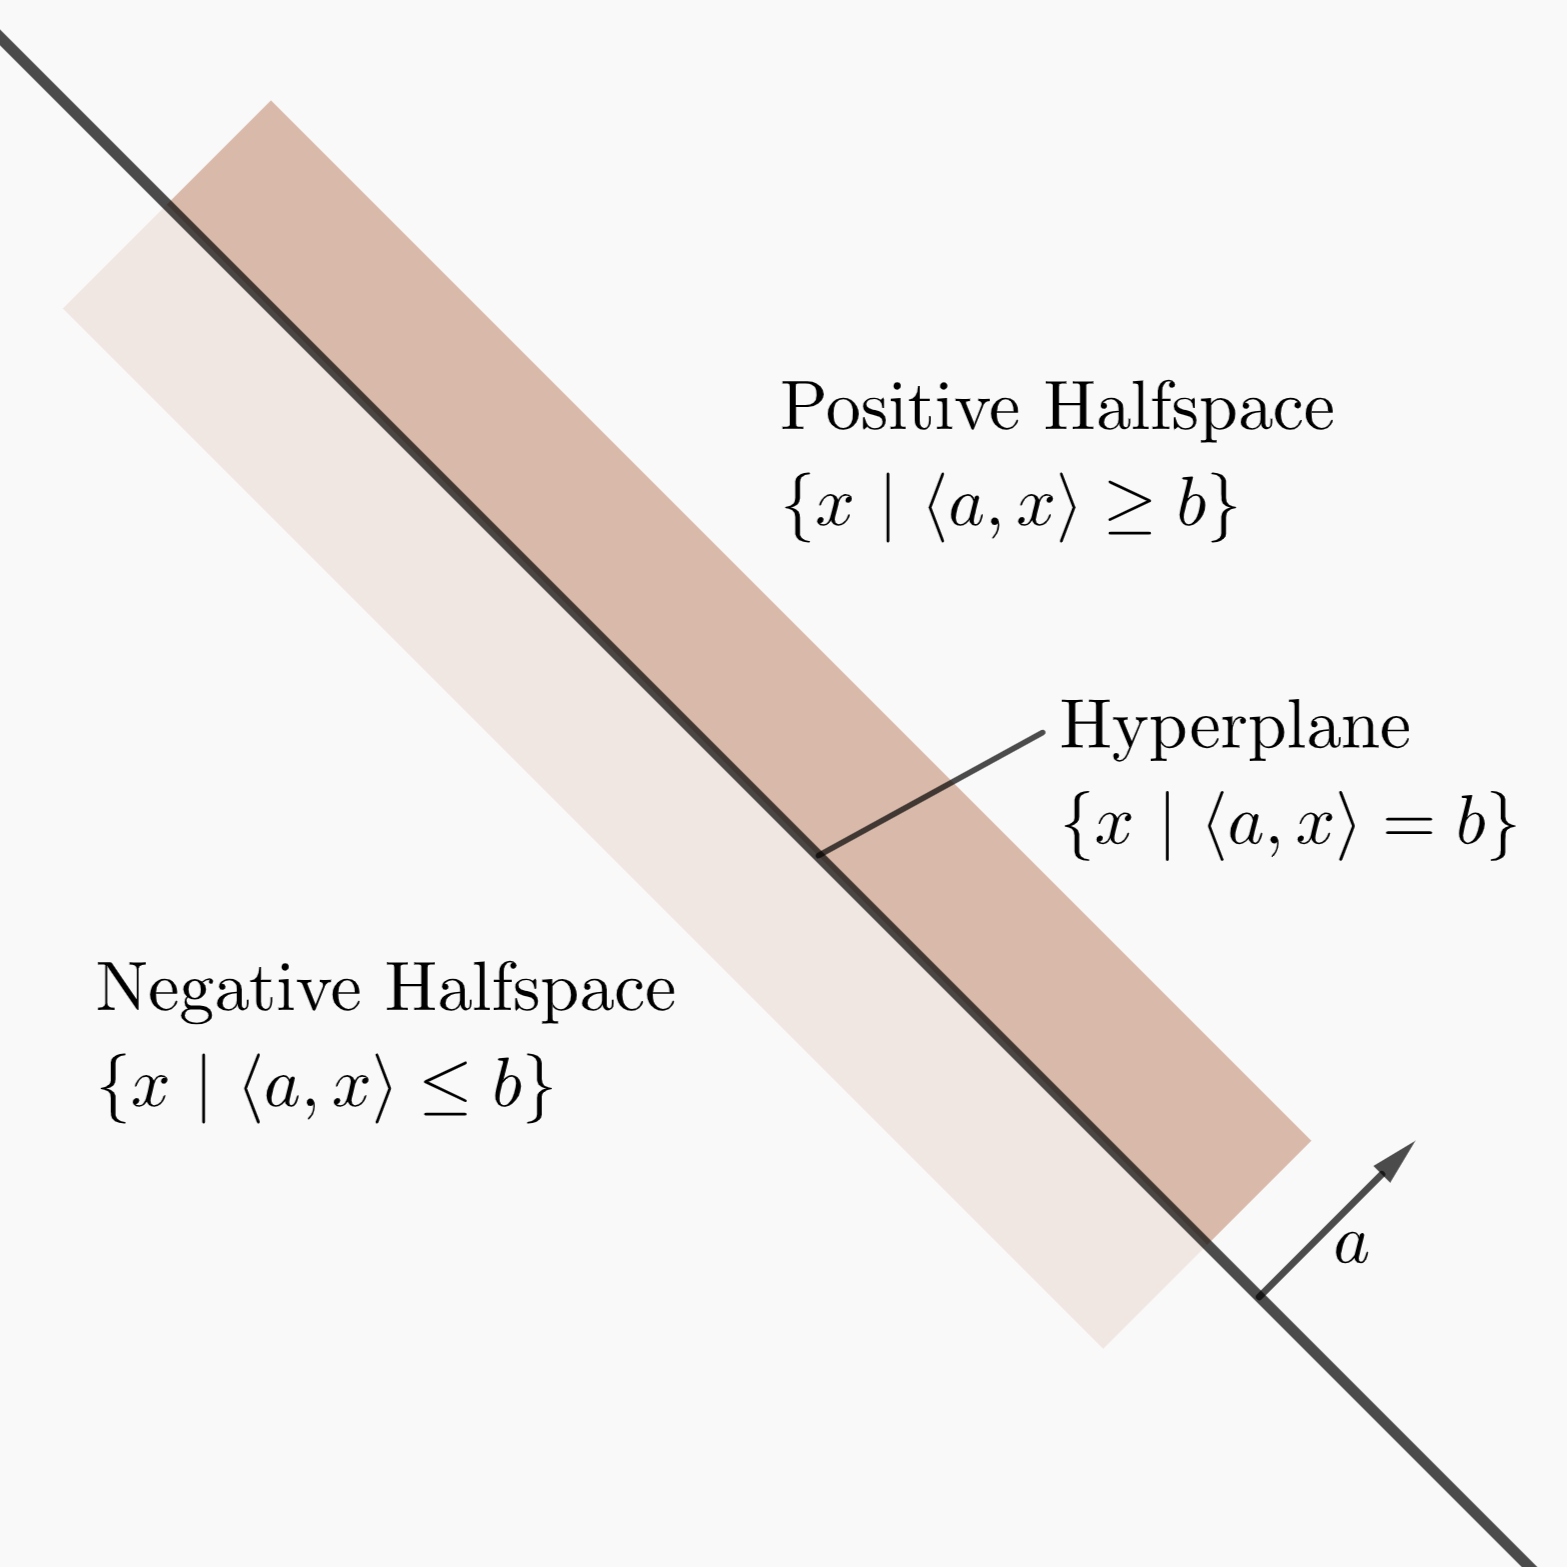
\includegraphics[height = 1.7 in]{halfspaces.png}
  \captionof{figure}{Closed Halfspaces}
  \label{fig:test1}
\end{minipage}%
\begin{minipage}{.5\textwidth}
  \centering
  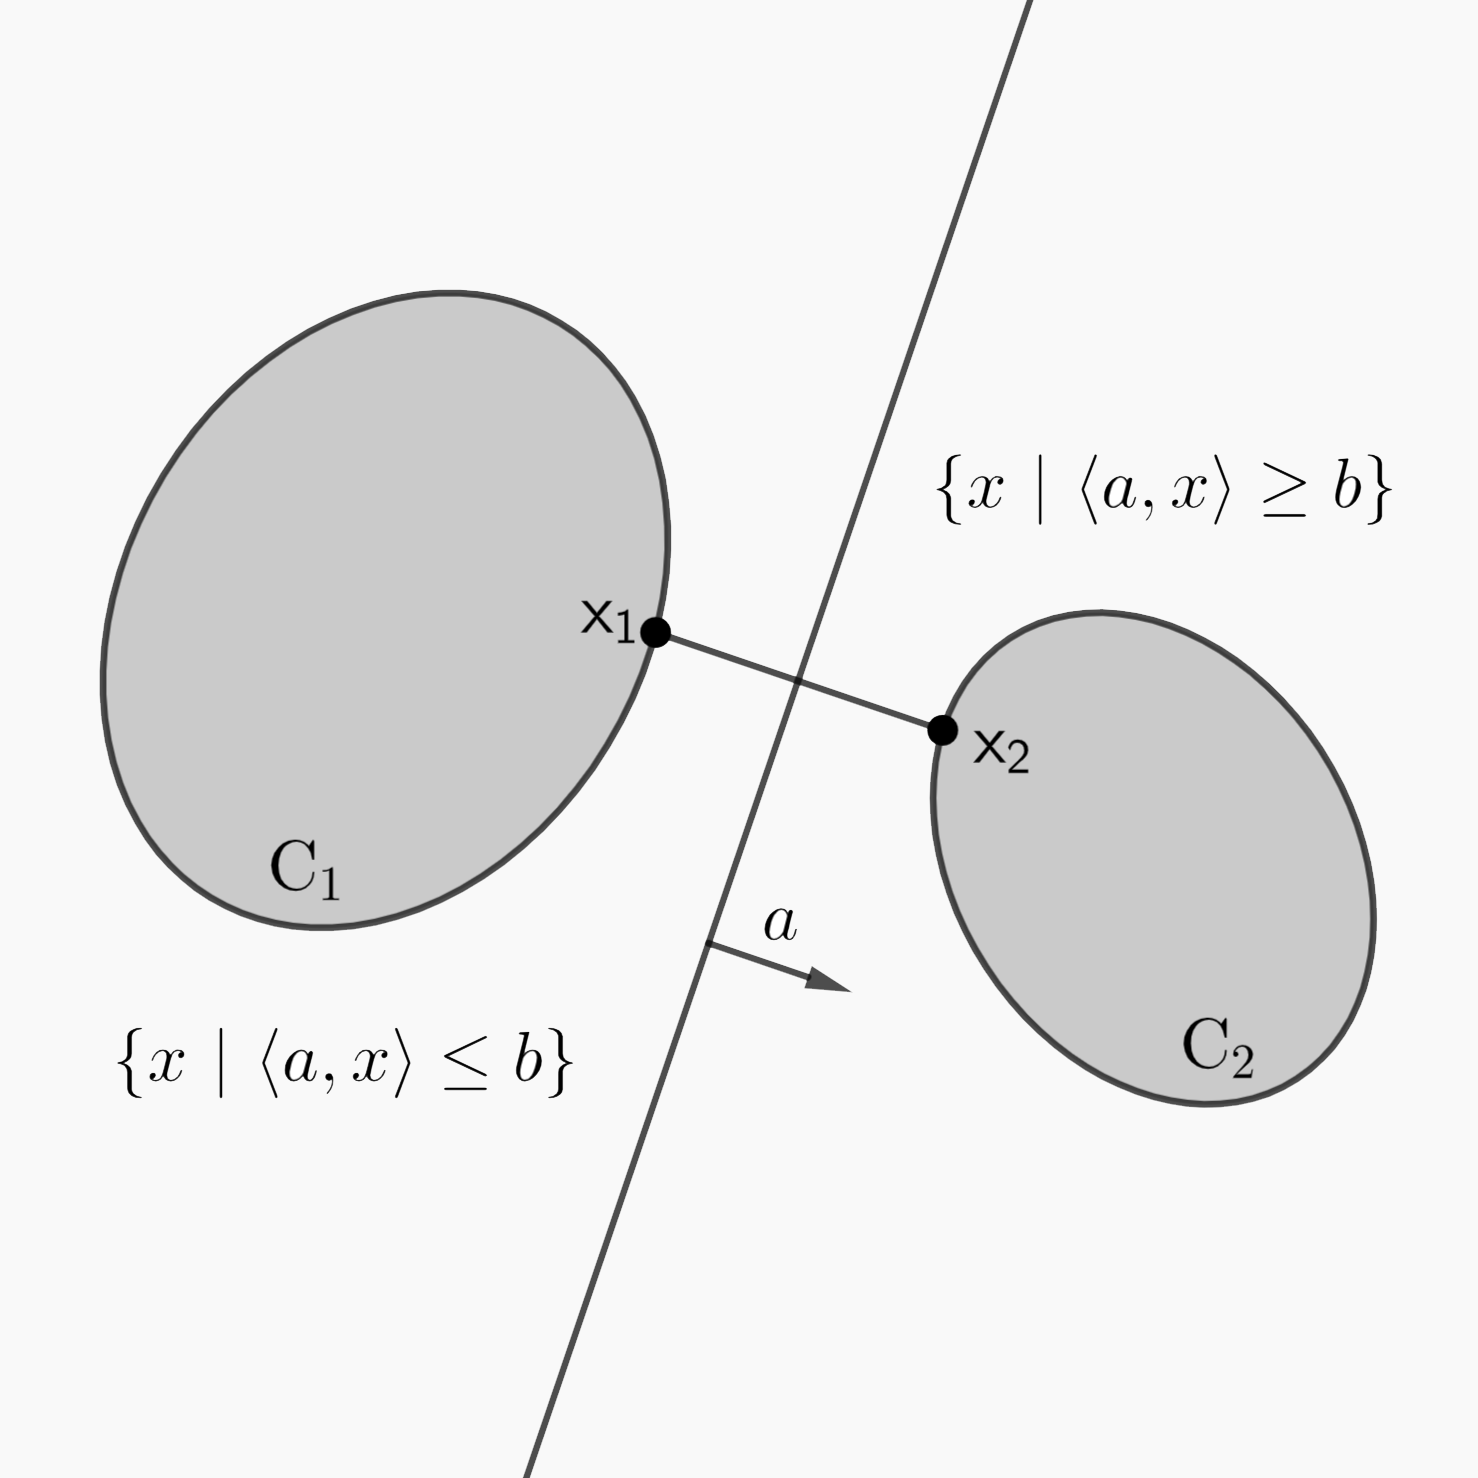
\includegraphics[height = 1.7 in]{separating hyperplane.png}
  \captionof{figure}{Sep. Hyperplane}
  \label{fig:test2}
\end{minipage}
\end{figure}
\end{example}
The notion of convexity is imbued throughout many different branches of mathematics, with myriad applications ranging from functional analysis, complex analysis, calculus, graph theory, partial differential equations, discrete mathematics, algebraic geometry, probability theory, coding theory, crystallography, etc. The study of convex optimization has grown in popularity as modern advances have spurred new applications of the field into existence. Uses of convex optimization range from estimation and signal processing, finance, statistics, automatic control systems, data modeling, and communication networks.\cite{boyd_vandenberghe_2004}  Specifically, separating hyperplanes have extensive applications in collision detection algorithms, ranging from computer simulations of physical bodies to collision avoidance in autonomous vehicles.\cite{mercy}
{
\setlength{\parskip}{8pt}
The history of Theorem \ref{thm:main} can be traced back to the ancient Greeks, Egyptians, and Babylonians, who first contemplated the notion of convexity. It was known to the ancient Greeks that only five regular convex polyhedra existed: the five Platonic solids. In his treatise \emph{On the Sphere and Cylinder}, Archimedes offered a more robust definition of convexity. He asserted that if a curve is drawn, if any line connecting two points on the curve falls exclusively on one side of the curve, it is concave on that side. Archimedes laid the foundation of convexity theory with many postulates relating to convex arcs, but they remained untouched for nearly two thousand years after their creation.\cite{roman}

In the 1840s, Augustin Louis Cauchy demonstrated thorough proofs of Archimedes's earlier postulates. He proved relations relating to curves, surface areas, and infinite sequences. These accomplishments occurred in tandem with the discovery of \emph{Euler's Formula}, which was proven by Adrien-Marie Legendre, and asserted that the number of vertices equals the number of edges in convex regular polyhedra.\cite{roman}

The modern definition of convexity has been shaped greatly by the work of Hermann Minkowski. His original interest in number theory led him to convex analysis, in part because he needed theorems relating to convex structures for his proofs. He specialized in isoperimetric problems, which aimed to determine the maxima or minima of geometric shapes under certain conditions; his work largely follows the isoperimetric inequality, which relates the perimeter and volume of convex structures. In his book, \emph{Geometry of Numbers}, Minkowski analyzes systems of the form $Ax \geq 0$, where $A$ is an $m x n$ matrix and $x$ is a vector, which are at the heart of linear programming problems. Minkowski forged the concepts of \emph{convex hulls} and \emph{extreme points}, points that can be removed from a convex set while preserving its state of being convex. The most relevant pieces of Minkowski's work to this paper include his \emph{distance function}, \emph{norms}, and the \emph{Hahn-Banach Theorem}, which is a generalization of the theorem presented in this paper.\cite{roman}

The structure of this paper is as follows. In section \ref{sec:background}, we give the necessary definitions of inner product spaces, lines and line-segments, affine and convex sets, hyperplanes, separation, and the Projection Theorem. Section \ref{sec:maintheorem} presents a proof of Theorem \ref{thm:main}, the Separating Hyperplane Theorem. In section \ref{sec:applications}, we demonstrate an application of Theorem \ref{thm:main}, and finally in section \ref{sec:futuredirections}, we present a couple of questions which are relevant to the applicability of Theorem \ref{thm:main}.

\subsection*{Acknowledgements} I would like to thank Professor Madeline Brandt for her course in Linear Algebra which laid the foundation for this paper, and for her insight during office hours. I would also like to thank my peer review partner during class for her valuable feedback.
}
%%%%%%%%%%%%%%%%%%%% BACKGROUND %%%%%%%%%%%%%%%%%%%%

\section{Background}
\label{sec:background}
{
\setlength{\parskip}{8pt}
We assume the reader is familiar with the fundamentals of fields, vector spaces, linear combinations, and dot products. We will begin by defining \emph{inner product spaces}, within which exists the \emph{inner product} operation between two vectors. Inner products can be utilized to define \emph{norms}, allowing us to convey a sense of distance within the vector space. Afterwards, we will define two methods of connecting points in space, namely \emph{lines} and \emph{line segments}. We will also define \emph{affine and convex combinations}, which are linear combinations of multiple points within a space. Together, these connections and combinations can be employed to define \emph{affine sets} and \emph{convex sets}, which are special forms of sets that contain all possible connections between their points. Afterwards, we will be able to define the \emph{relative interior}, \emph{closure}, and \emph{relative boundaries} of sets. Finally, this will lead us to the definitions of \emph{hyperplanes} and the concept of \emph{separation} between two convex sets, which is the primary subject of Theorem \ref{thm:main}.
\smallskip
\begin{definition}[{Inner Product Space, \cite{nimark}}]
    Consider a vector space $V$. $V$ is an \emph{inner product space} if there exists a scalar $\langle x,y\rangle$ called an \emph{inner product} for each pair of elements $x,y\in V$ such that the following three conditions hold:

    (note: a bar over a scalar represents its \emph{complex conjugate}; \emph{i.e.} the complex conjugate of a scalar $a + bi$ where $a,b\in\R$ is $a - bi$)

    (1) Conjugate Symmetry
    \begin{align*}
        \langle x,y\rangle &= \overline{\langle y,x\rangle} &\text{for all $x,y\in V$}
    \end{align*}
    (2) Linearity
    \begin{align*}
        \langle x+z,y\rangle &= \langle x,y\rangle + \langle z,y\rangle & \text{for all $x,y,z\in V$}\\
         \langle \alpha x,y\rangle &= \alpha\langle x,y\rangle &\text{for all $x,y\in V$ and $\alpha\in\R$}
    \end{align*}
    (3) Positive Definiteness
    \begin{align*}
        \langle x,x\rangle &> 0 \text{ if and only if } x\neq 0 &\text{for all $x\in V$}\\
        \langle x,x\rangle &= 0 \text{ if and only if } x=0 &\text{for all $x\in V$}
    \end{align*}

    The real n-space, denoted $\R^n$, is an example of an inner product space in which the \emph{dot product} serves as the inner product operation.
\end{definition}
\smallskip
\begin{example}
    We will now give examples of each of these properties for vectors in $\R^3$.

    (1) Conjugate Symmetry
    \begin{align*}
        \langle (1, 3, 2), (5, 2, 4)\rangle &= \overline{\langle (5, 2, 4), (1, 3, 2)\rangle}\\
        1\cdot 5 + 3\cdot 2 + 2\cdot 4 &= 5\cdot 1 + 2\cdot 3 + 4\cdot 2\\
        5 + 6 + 8 &= 5 + 6 + 8\\
        19 &= 19
    \end{align*}
    (2) Linearity
    \begin{align*}
        \langle (7, 6, 6) + (1, 4, 8), (5, 5, 1)\rangle &= \langle (7, 6, 6),(5, 5, 1)\rangle + \langle (1, 4, 8),(5, 5, 1)\rangle\\
        5(7+1) + 5(6+4) + 1(6+8) &= 7\cdot 5 + 6\cdot 5 + 6\cdot 1 + 1\cdot 5 + 4\cdot 5 + 8\cdot 1\\
        40 + 50 + 14 &= 35 + 30 + 6 + 5 + 20 + 8\\
        104 &= 104
    \end{align*}
    \begin{align*}
        \langle6(4, 5, 2),(7, 7, 7)\rangle &= 6\langle(4,5,2),(7,7,7)\rangle\\
        24\cdot 7 + 30\cdot 7 + 12\cdot 7 &= 6(4\cdot 7 + 5\cdot 7 + 2\cdot 7)\\
        462 &= 462
    \end{align*}
    (3) Positive Definiteness
    \begin{align*}
        \langle (1, 1, 1), (1, 1, 1)\rangle &= 1 + 1 + 1\\
        &> 0
    \end{align*}
    \begin{align*}
        \langle (0,0,0),(0,0,0)\rangle &= 0 + 0 + 0\\
        &= 0
    \end{align*}
\end{example}
\smallskip
\begin{definition}[{Norms, \cite{nimark}}]
    Let $v\in V$ such that $V$ is an inner product space. We define the length, or \emph{norm}, of $v$ as
    \begin{align*}
        ||v|| = \sqrt{\langle v,v\rangle}
    \end{align*}
    In other words, the inner product of a vector with itself is its norm squared, as follows
    \begin{align*}
        \langle v,v\rangle = ||v||^2
    \end{align*}
\end{definition}
\smallskip
\begin{example}
    Consider the vector $(4, 2, 7)$ in $\R^3$. The norm of this vector can be expressed as
    \begin{align*}
        \sqrt{\langle(4,2,7),(4,2,7)\rangle}&= \sqrt{16+4+49}\\
        &= \sqrt{69}
    \end{align*}
\end{example}
\smallskip
\begin{definition}[{Lines and Line Segments, \cite[2.1.1]{boyd_vandenberghe_2004}}]
    Let $x_1 \neq x_2$ be two points in $\R^n$. Points defined by
    \begin{align*}
        y = x_2 + \theta(x_1 - x_2)
    \end{align*}
    form a connection between $x_1$ and $x_2$. A \emph{line-segment} between $x_1$ and $x_2$ is defined as the set of $y$ such that $0 \leq \theta \leq 1$. A \emph{line} through $x_1$ and $x_2$ is defined as the set of all $y$ such that $\theta \in \R$. This relationship can also be expressed as
    \begin{align*}
        y = \theta x_1 + (1 - \theta)x_2
    \end{align*}
    \emph{i.e.} a combination of $x_1$ and $x_2$ in which the coefficients total $1$.
\end{definition}
\smallskip
\begin{example}
    Consider the line and line segment connecting the points $(-1,-1)$ and $(2,3)$ in $\R^2$.
    \begin{figure}[h]
    \centering
    \begin{minipage}{.5\textwidth}
      \centering
      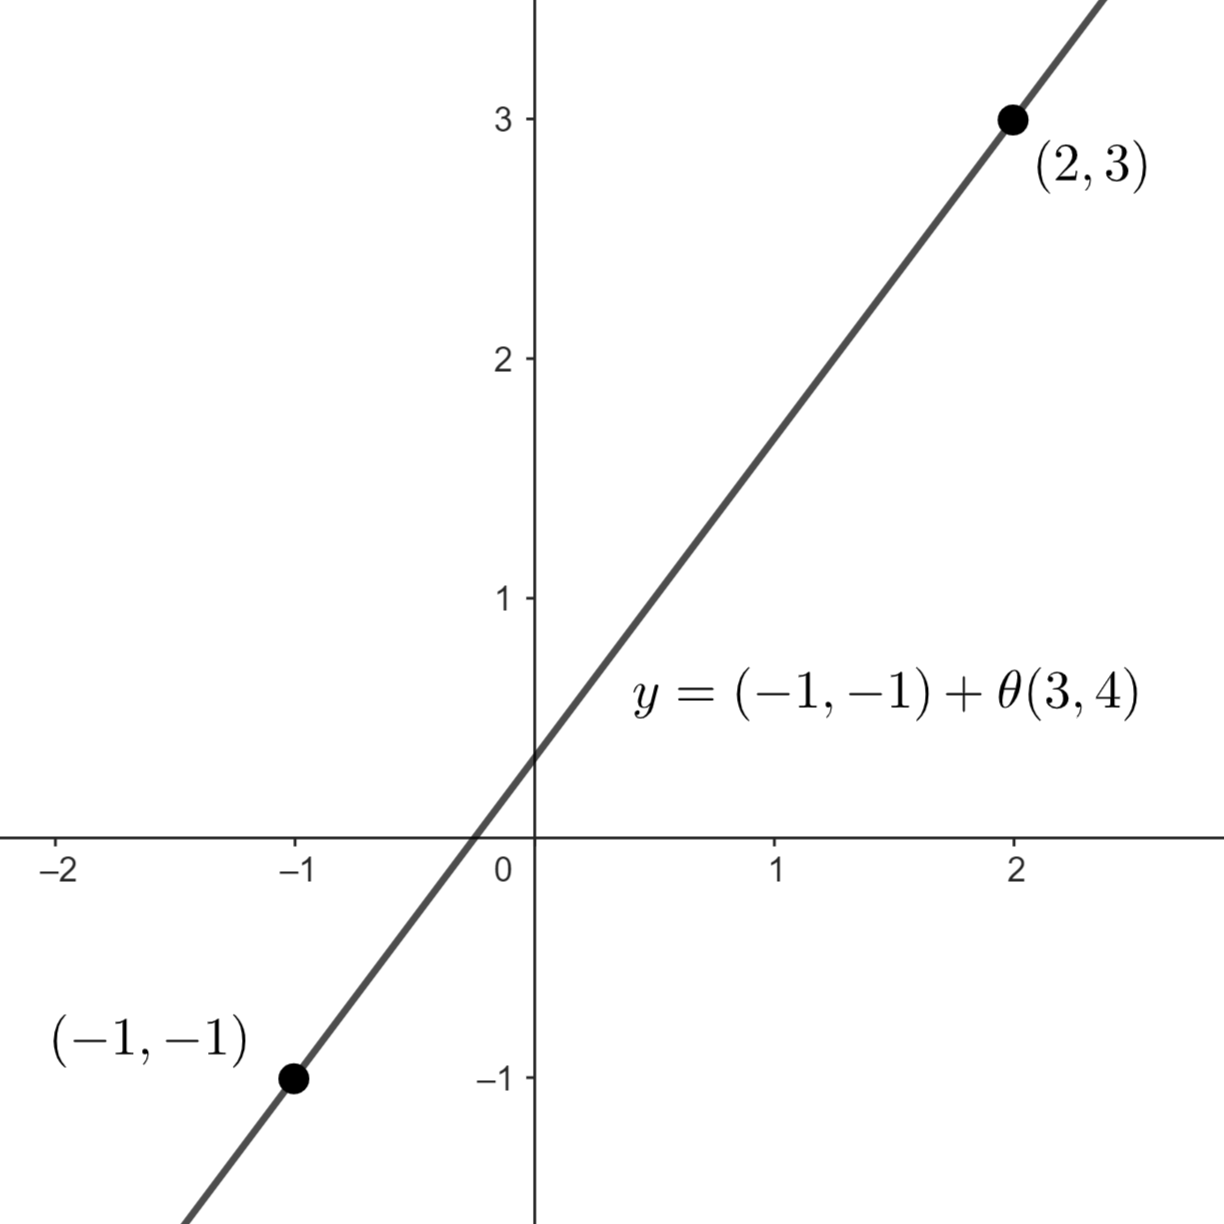
\includegraphics[height = 1.7 in]{Line.png}
      \captionof{figure}{Line}
      \label{fig:test1}
    \end{minipage}%
    \begin{minipage}{.5\textwidth}
      \centering
      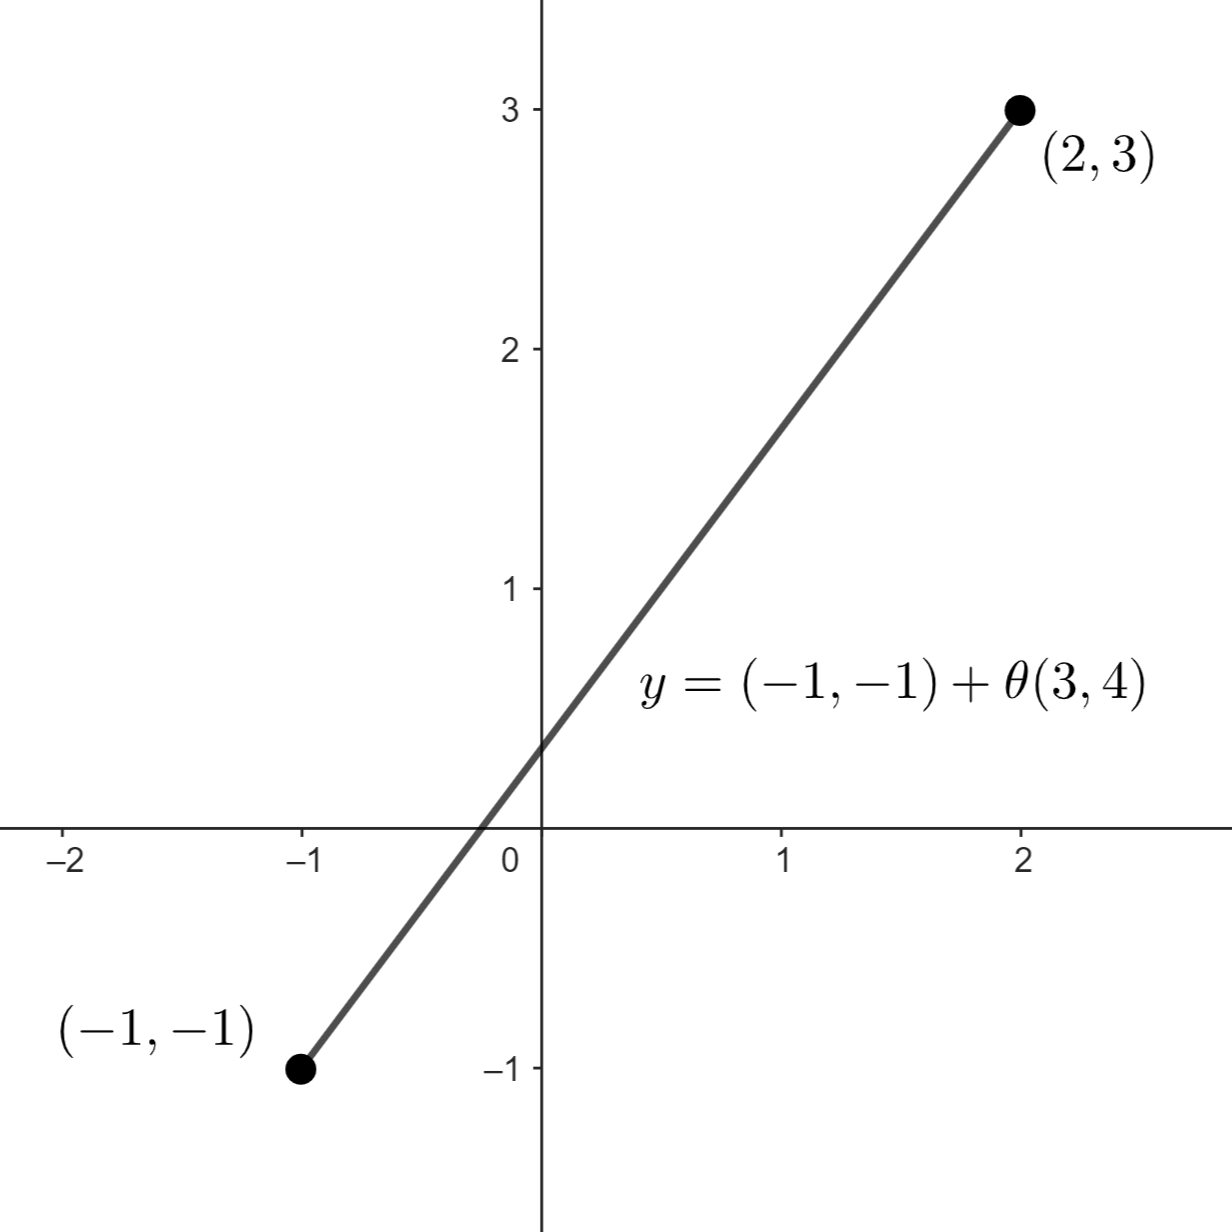
\includegraphics[height = 1.7 in]{segment.png}
      \captionof{figure}{Line Segment}
      \label{fig:test2}
    \end{minipage}
    \end{figure}
\end{example}
\smallskip
\begin{definition}[{Affine Combinations, \cite[2.1.2]{boyd_vandenberghe_2004}}]
    Let $x_1,\ldots,x_k$ be points in $\R^n$, and let $\theta_1+\cdots+\theta_k=1$. An \emph{affine-combination} of $x_1,\ldots,x_k$ is a point formed by the linear combination $\theta_1x_1+\cdots+\theta_kx_k$.
\end{definition}
\smallskip
\begin{definition}[{Convex Combinations, \cite[2.1.4]{boyd_vandenberghe_2004}}]
    Let $x_1,\ldots,x_k$ be points in $\R^n$, and let $\theta_1,\ldots,\theta_k\in\R$ such that $\theta_i\geq 0$ and $\theta_1+\cdots+\theta_k=1$. A point formed by the linear combination $\theta_1x_1+\cdots+\theta_kx_k$ is called a \emph{convex combination}.
\end{definition}
\smallskip
\begin{definition}[{Affine Sets, \cite[2.1.2]{boyd_vandenberghe_2004}}]
    Let $C \subseteq \R^n$ be a set of points. $C$ is \emph{affine} if the line through any two points, $x_1, x_2 \in C$, is fully contained within $C$:
    \begin{align*}
        \theta x_1 + (1 - \theta)x_2 \in C \text{ for all } \theta\in\R
    \end{align*}
    In other words, an \emph{affine set} is a set that contains every possible affine combination of its points. Therefore, if $x_1,\ldots,x_k\in C$, and $\theta_1+\cdots+\theta_k=1$, $\theta_1x_1+\cdots+\theta_kx_k\in C$.

    By Lemma \ref{lem:aff}, an \emph{affine set} C can be expressed as
    \begin{align*}
        C = V + x_0 = \{v + x_0\ |\ v\in V\}
    \end{align*}
    \emph{i.e.} as a subspace $V$ of $\R^n$ plus an offset $x_0$. The subspace, $V$, corresponding to $C$ is not dependent on the choice of $x_0$, as long as $x_0\in C$.
\end{definition}
\smallskip
\begin{example}
    Lines and planes are both examples of affine sets. The line connecting any two points within these structures will always be fully contained within the set.
    \begin{figure}[h]
    \centering
    \begin{minipage}{.5\textwidth}
      \centering
      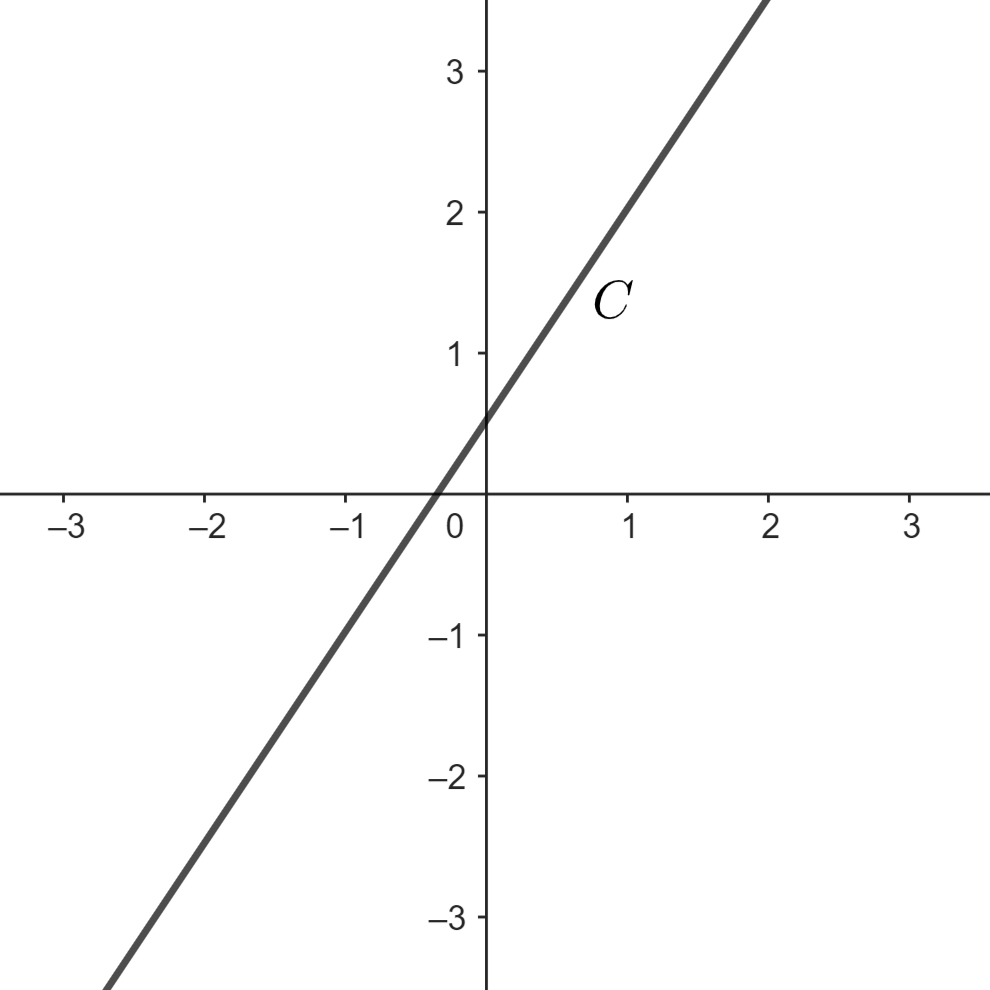
\includegraphics[height = 1.7 in]{affine2.png}
      \captionof{figure}{Affine Line}
      \label{fig:test1}
    \end{minipage}%
    \begin{minipage}{.5\textwidth}
      \centering
      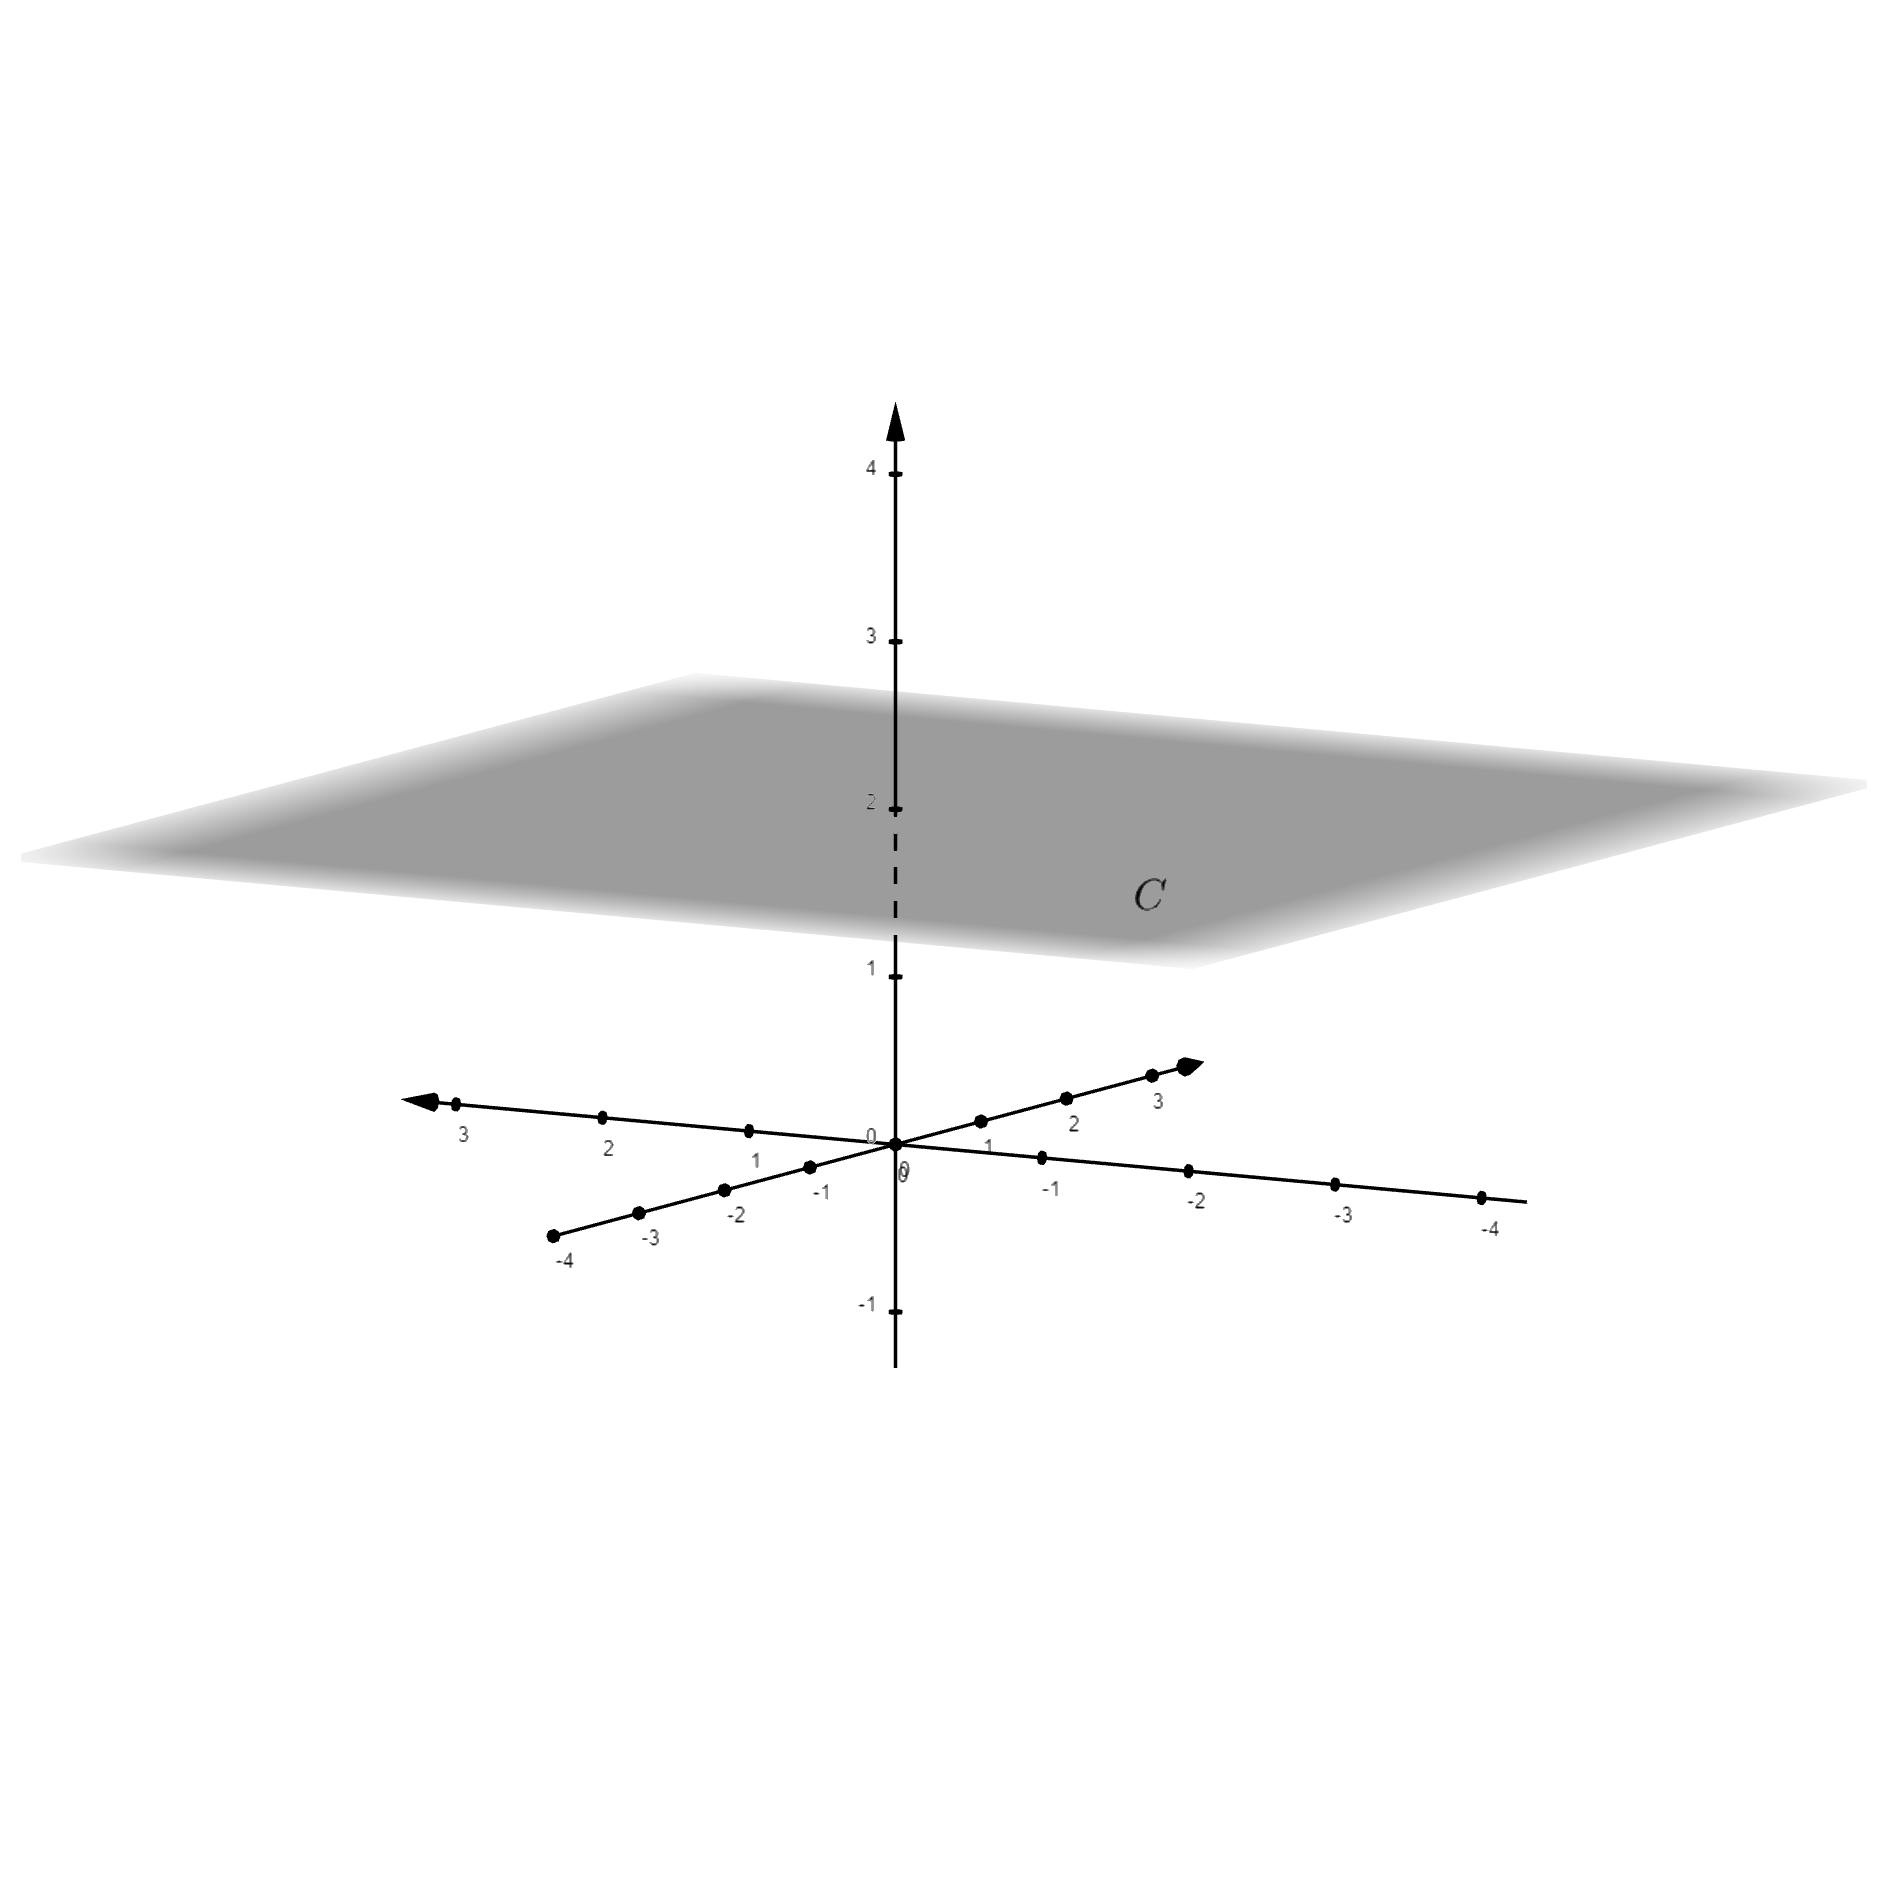
\includegraphics[height = 1.7 in]{affineset.png}
      \captionof{figure}{Affine Plane}
      \label{fig:test2}
    \end{minipage}
    \end{figure}
\end{example}
\smallskip
\begin{lemma} 
    \label{lem:aff}
    Let $x_0 \in C$. If $C$ is an affine set, then the set
    \begin{align*}
        V = C - x_0 = \{x - x_0\ |\ x\in C\}
    \end{align*}
    is a subspace, which we will now prove. 
    \begin{proof}
        It immediately follows that $0\in V$ since $x_0-x_0=0$. It remains to prove that $V$ is closed over addition and scalar multiplication.
        
        Consider any two vectors $v_1,v_2 \in V$ and two scalars $\alpha,\beta\in\R$. It's given that $x_0 \in C$ and it follows that $v_1 + x_0 \in C$ and $v_2 + x_0 \in C$. Therefore,
        \begin{align*}
            \alpha v_1 + \beta v_2 + x_0 = \alpha(v_1 + x_0) + \beta(v_2 + x_0) + (1 - \alpha - \beta)x_0 \in C
        \end{align*}
        because $C$ is an affine set and $\alpha + \beta + (1 - \alpha - \beta) = 1$. Thus, $\alpha v_1 + \beta v_2 \in V$ since we have that $\alpha v_1 + \beta v_2 + x_0 \in C$. Therefore, $V$ is closed under addition.
        
        Additionally, let $v\in V$ and $\lambda\in\R$. Since $v = c - x_0$ for some $c\in C$, a scalar multiple of $v$ can be expressed as
        \begin{align*}
            \lambda v = \lambda c - \lambda x_0 = \lambda c - (\lambda - 1)x_0 - x_0 \in V
        \end{align*}
        Since $C$ is affine and $c,x_0\in C$ and $\lambda - (\lambda - 1) = 1$, we have that $\lambda c - (\lambda - 1)x_0\in C$. Therefore, $V$ is closed under scalar multiplication.
    \end{proof}
\end{lemma}
\smallskip
\begin{definition}[{Convex Sets, \cite[2.1.4]{boyd_vandenberghe_2004}}]
    Let $C\subseteq\R^n$ be a set of points. $C$ is \emph{convex} if the line-segment connecting any two points, $x_1,x_2\in C$, is fully contained within $C$:
    \begin{align*}
        \theta x_1 + (1 - \theta)x_2 \in C \text{ for all } 0 \leq \theta \leq 1
    \end{align*}
    In other words, a set $C$ is \emph{convex} if it contains every possible convex combination of its points.
\end{definition}
\smallskip
\begin{example}
    Consider the following examples and nonexamples of convex sets within $\R^2$. Given a set, if it is possible to construct a line-segment joining two points in the set such that the entire line segment is not fully contained within the set, then the set is not convex.
    \begin{figure}[h]
    \centering
    \begin{minipage}{.5\textwidth}
      \centering
      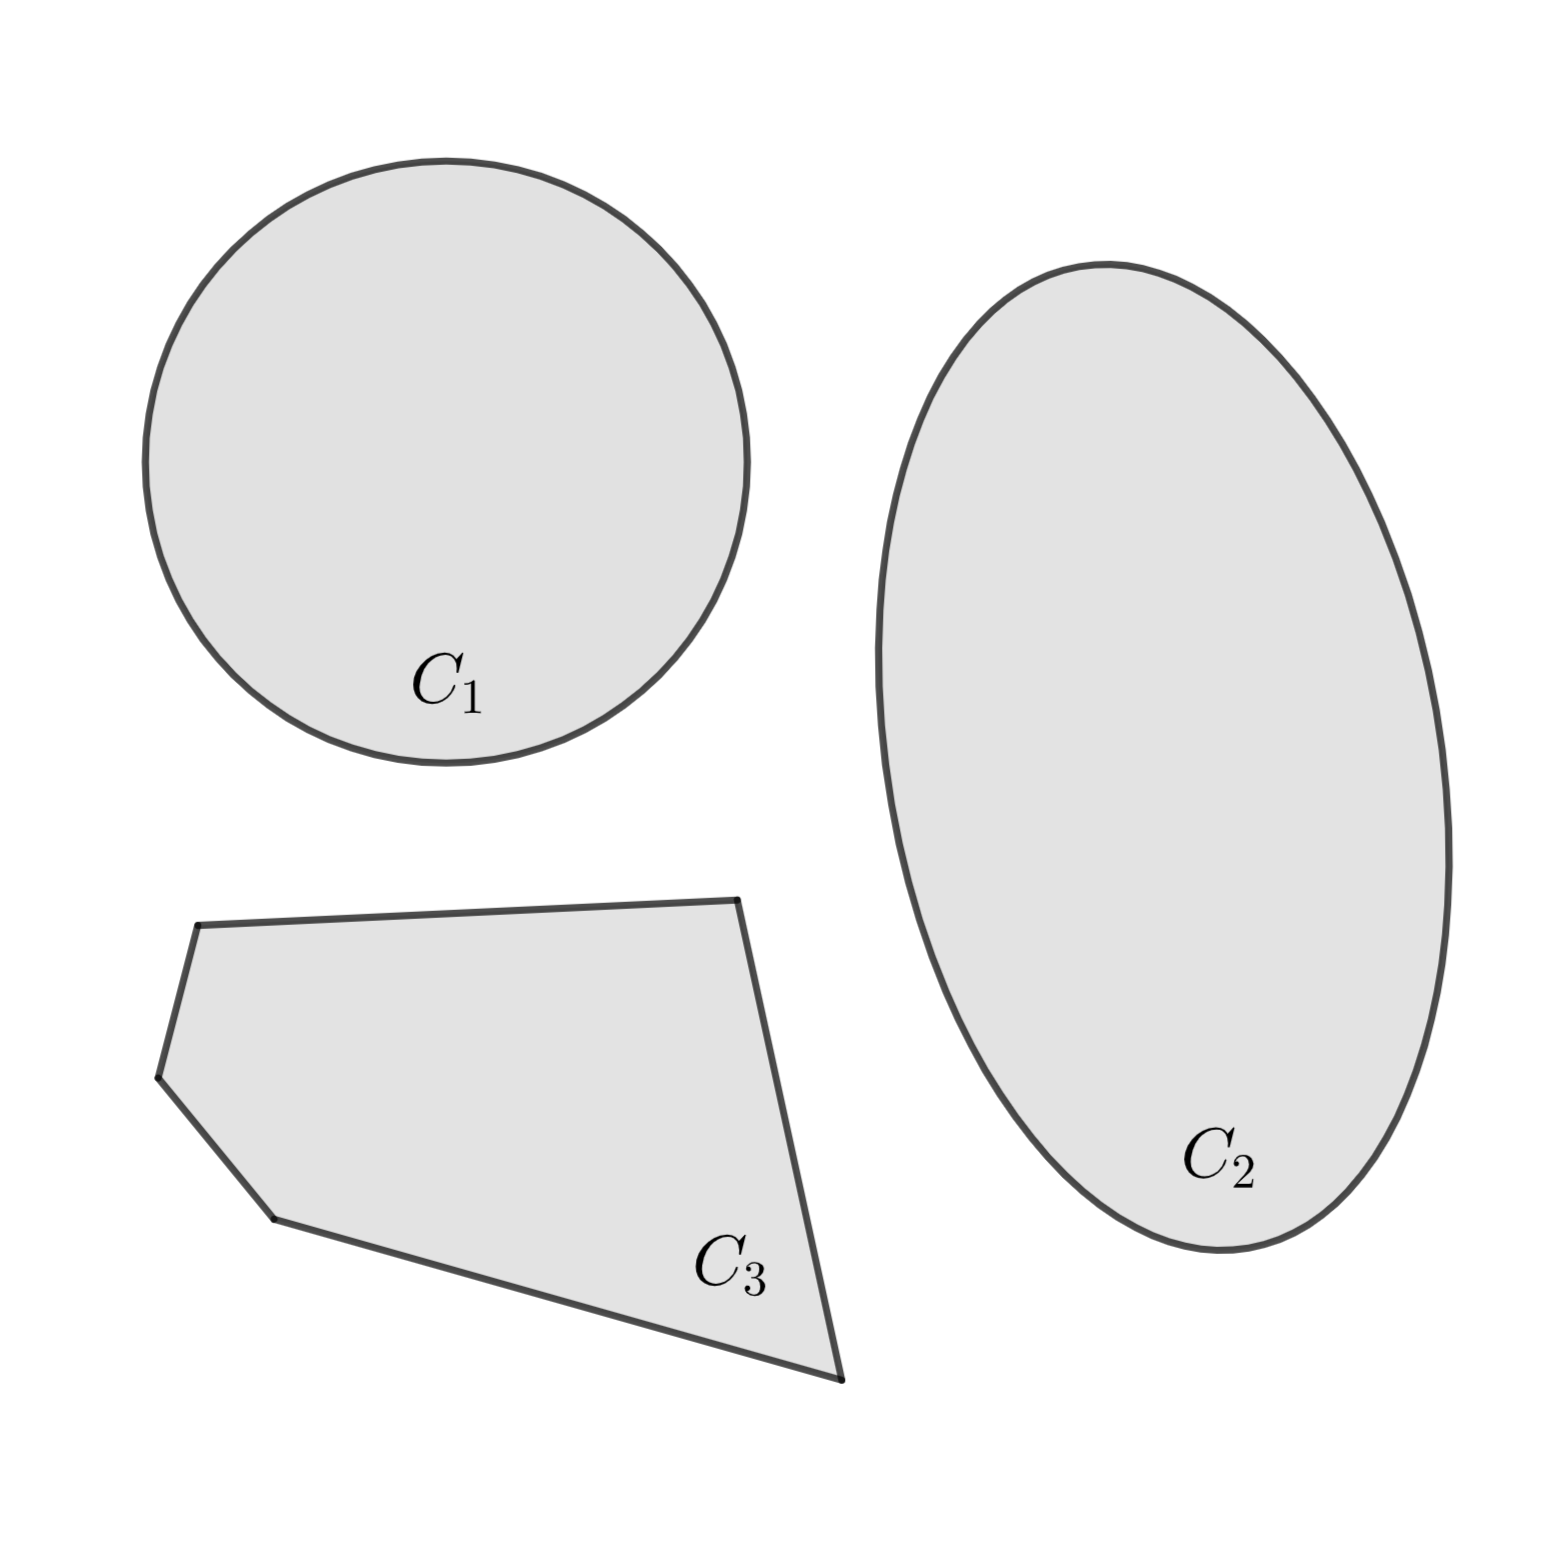
\includegraphics[height = 1.7 in]{convex.png}
      \captionof{figure}{Convex Sets}
      \label{fig:test1}
    \end{minipage}%
    \begin{minipage}{.5\textwidth}
      \centering
      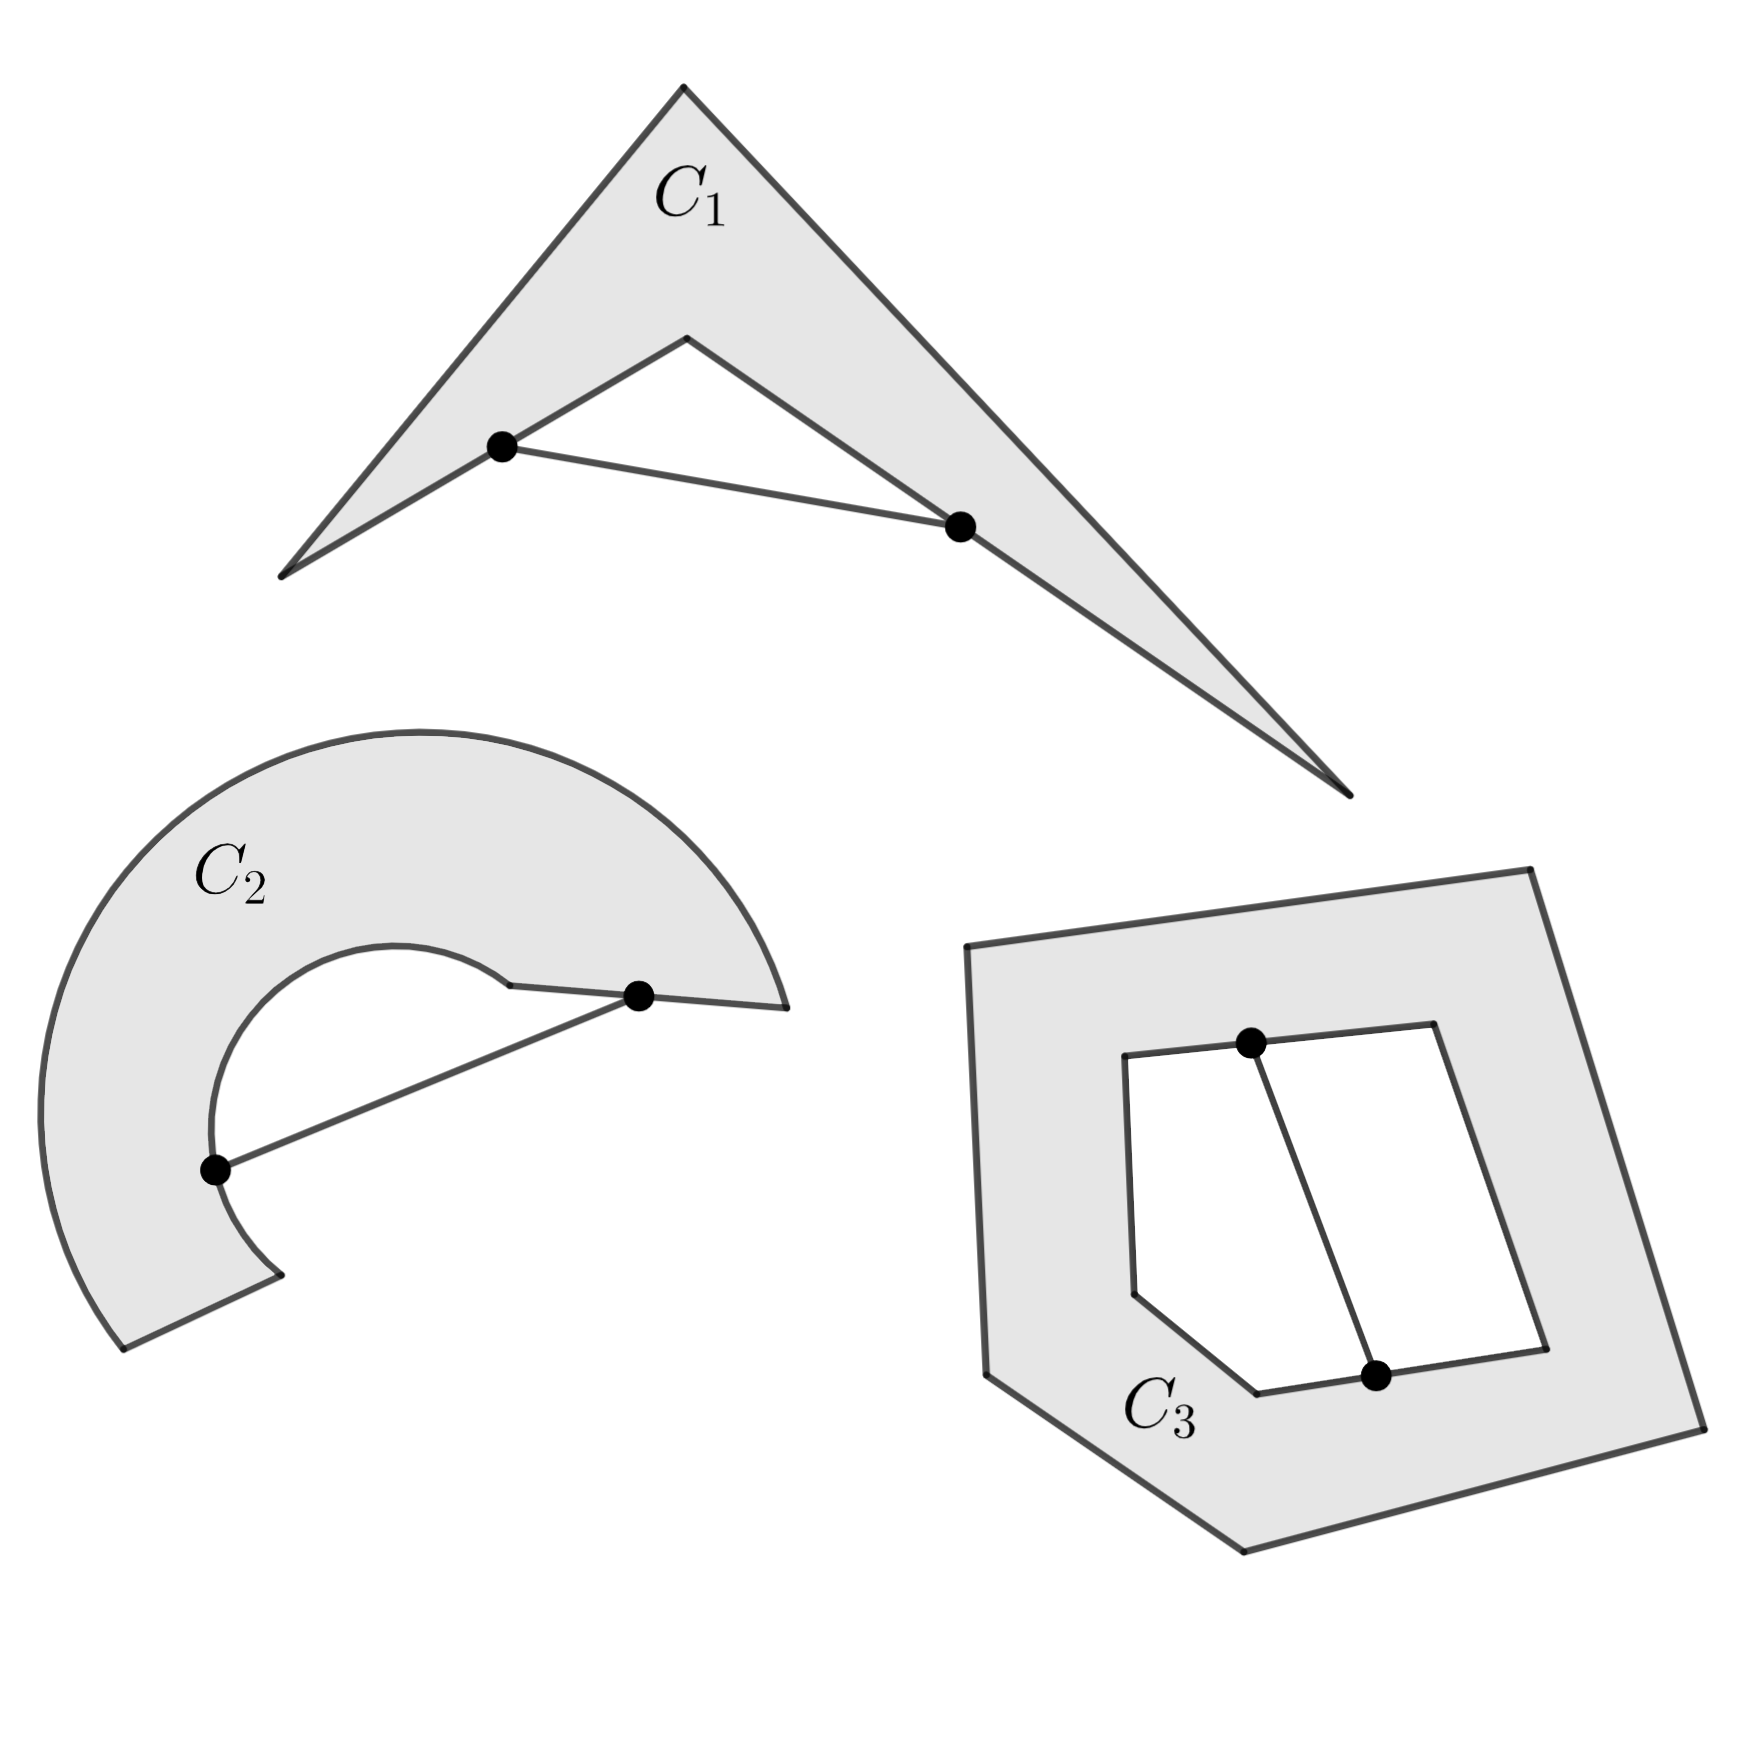
\includegraphics[height = 1.7 in]{notconvex.png}
      \captionof{figure}{Non-convex Sets}
      \label{fig:test2}
    \end{minipage}
    \end{figure}
\end{example}
\smallskip
\begin{definition}[{Affine Hulls, \cite[2.1.2]{boyd_vandenberghe_2004}}]
    Let $C\subseteq\R^n$ be a set. The \emph{affine hull} of $C$ is the set of all possible affine combinations of points in $C$, which can be expressed as
    \begin{align*}
        \aff C = \{\theta_1x_1+\cdots+\theta_kx_k\ |\ x_i\in C,\ \theta_1+\cdots+\theta_k=1\}
    \end{align*}
    \emph{i.e.} the smallest affine set containing $C$.
\end{definition}
\smallskip
\begin{definition}[{Convex Hulls, \cite[2.1.4]{boyd_vandenberghe_2004}}]
    Let $C\subseteq\R^n$ be a set. The \emph{convex hull} of $C$ is the set of all possible convex combinations of points in $C$, which can be expressed as
    \begin{align*}
        \conv C = \{\theta_1x_1+\cdots+\theta_kx_k\ |\ x_i\in C,\ \theta_i\geq 0,\ \theta_1+\cdots+\theta_k=1\}
    \end{align*}
    \emph{i.e.} the smallest convex set that contains $C$.
\end{definition}
\smallskip
\begin{example}
    Consider the following non-convex set $C$ in $\R^2$. The affine hull of $C$ is the entire vector space $\R^2$, as shown in the following figure on the left. Additionally, the convex hull of $C$ is the smallest convex set that contains all of $C$, as depicted in the figure on the right.
    \begin{figure}[h]
    \centering
    \begin{minipage}{.5\textwidth}
      \centering
      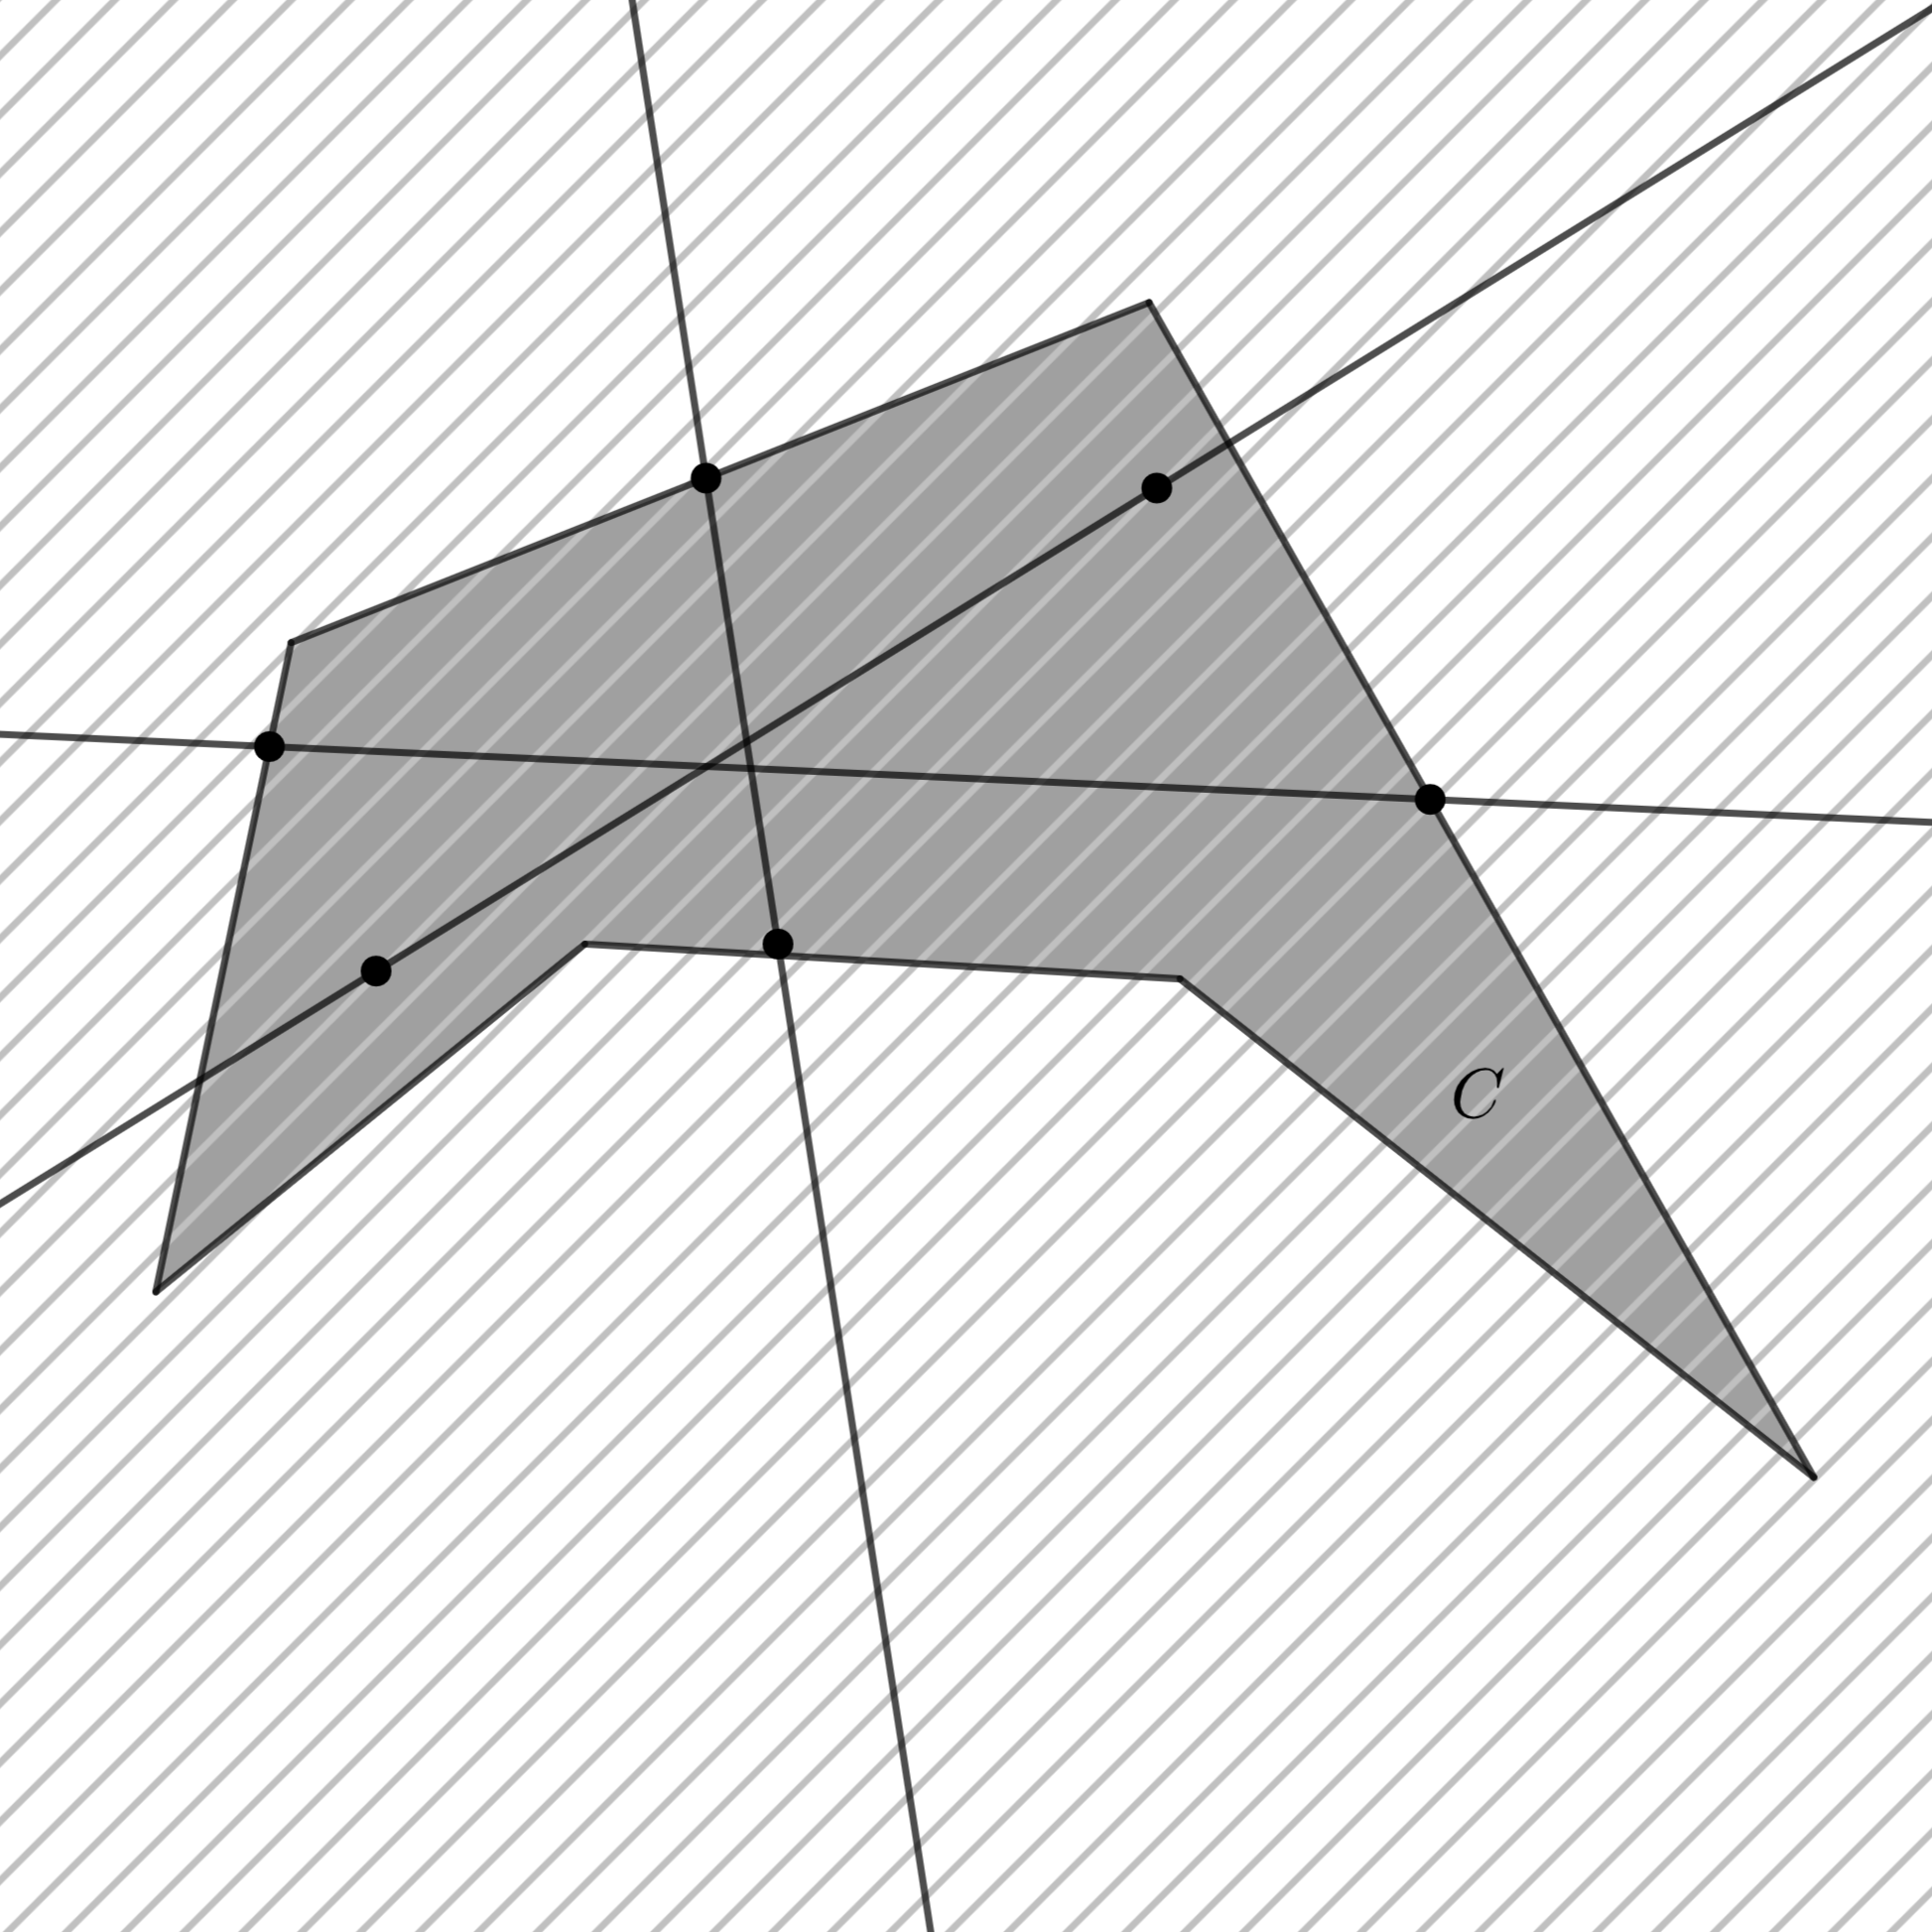
\includegraphics[height = 1.7 in]{AffineHull.png}
      \captionof{figure}{$\aff C$ is $\R^2$}
      \label{fig:test1}
    \end{minipage}%
    \begin{minipage}{.5\textwidth}
      \centering
      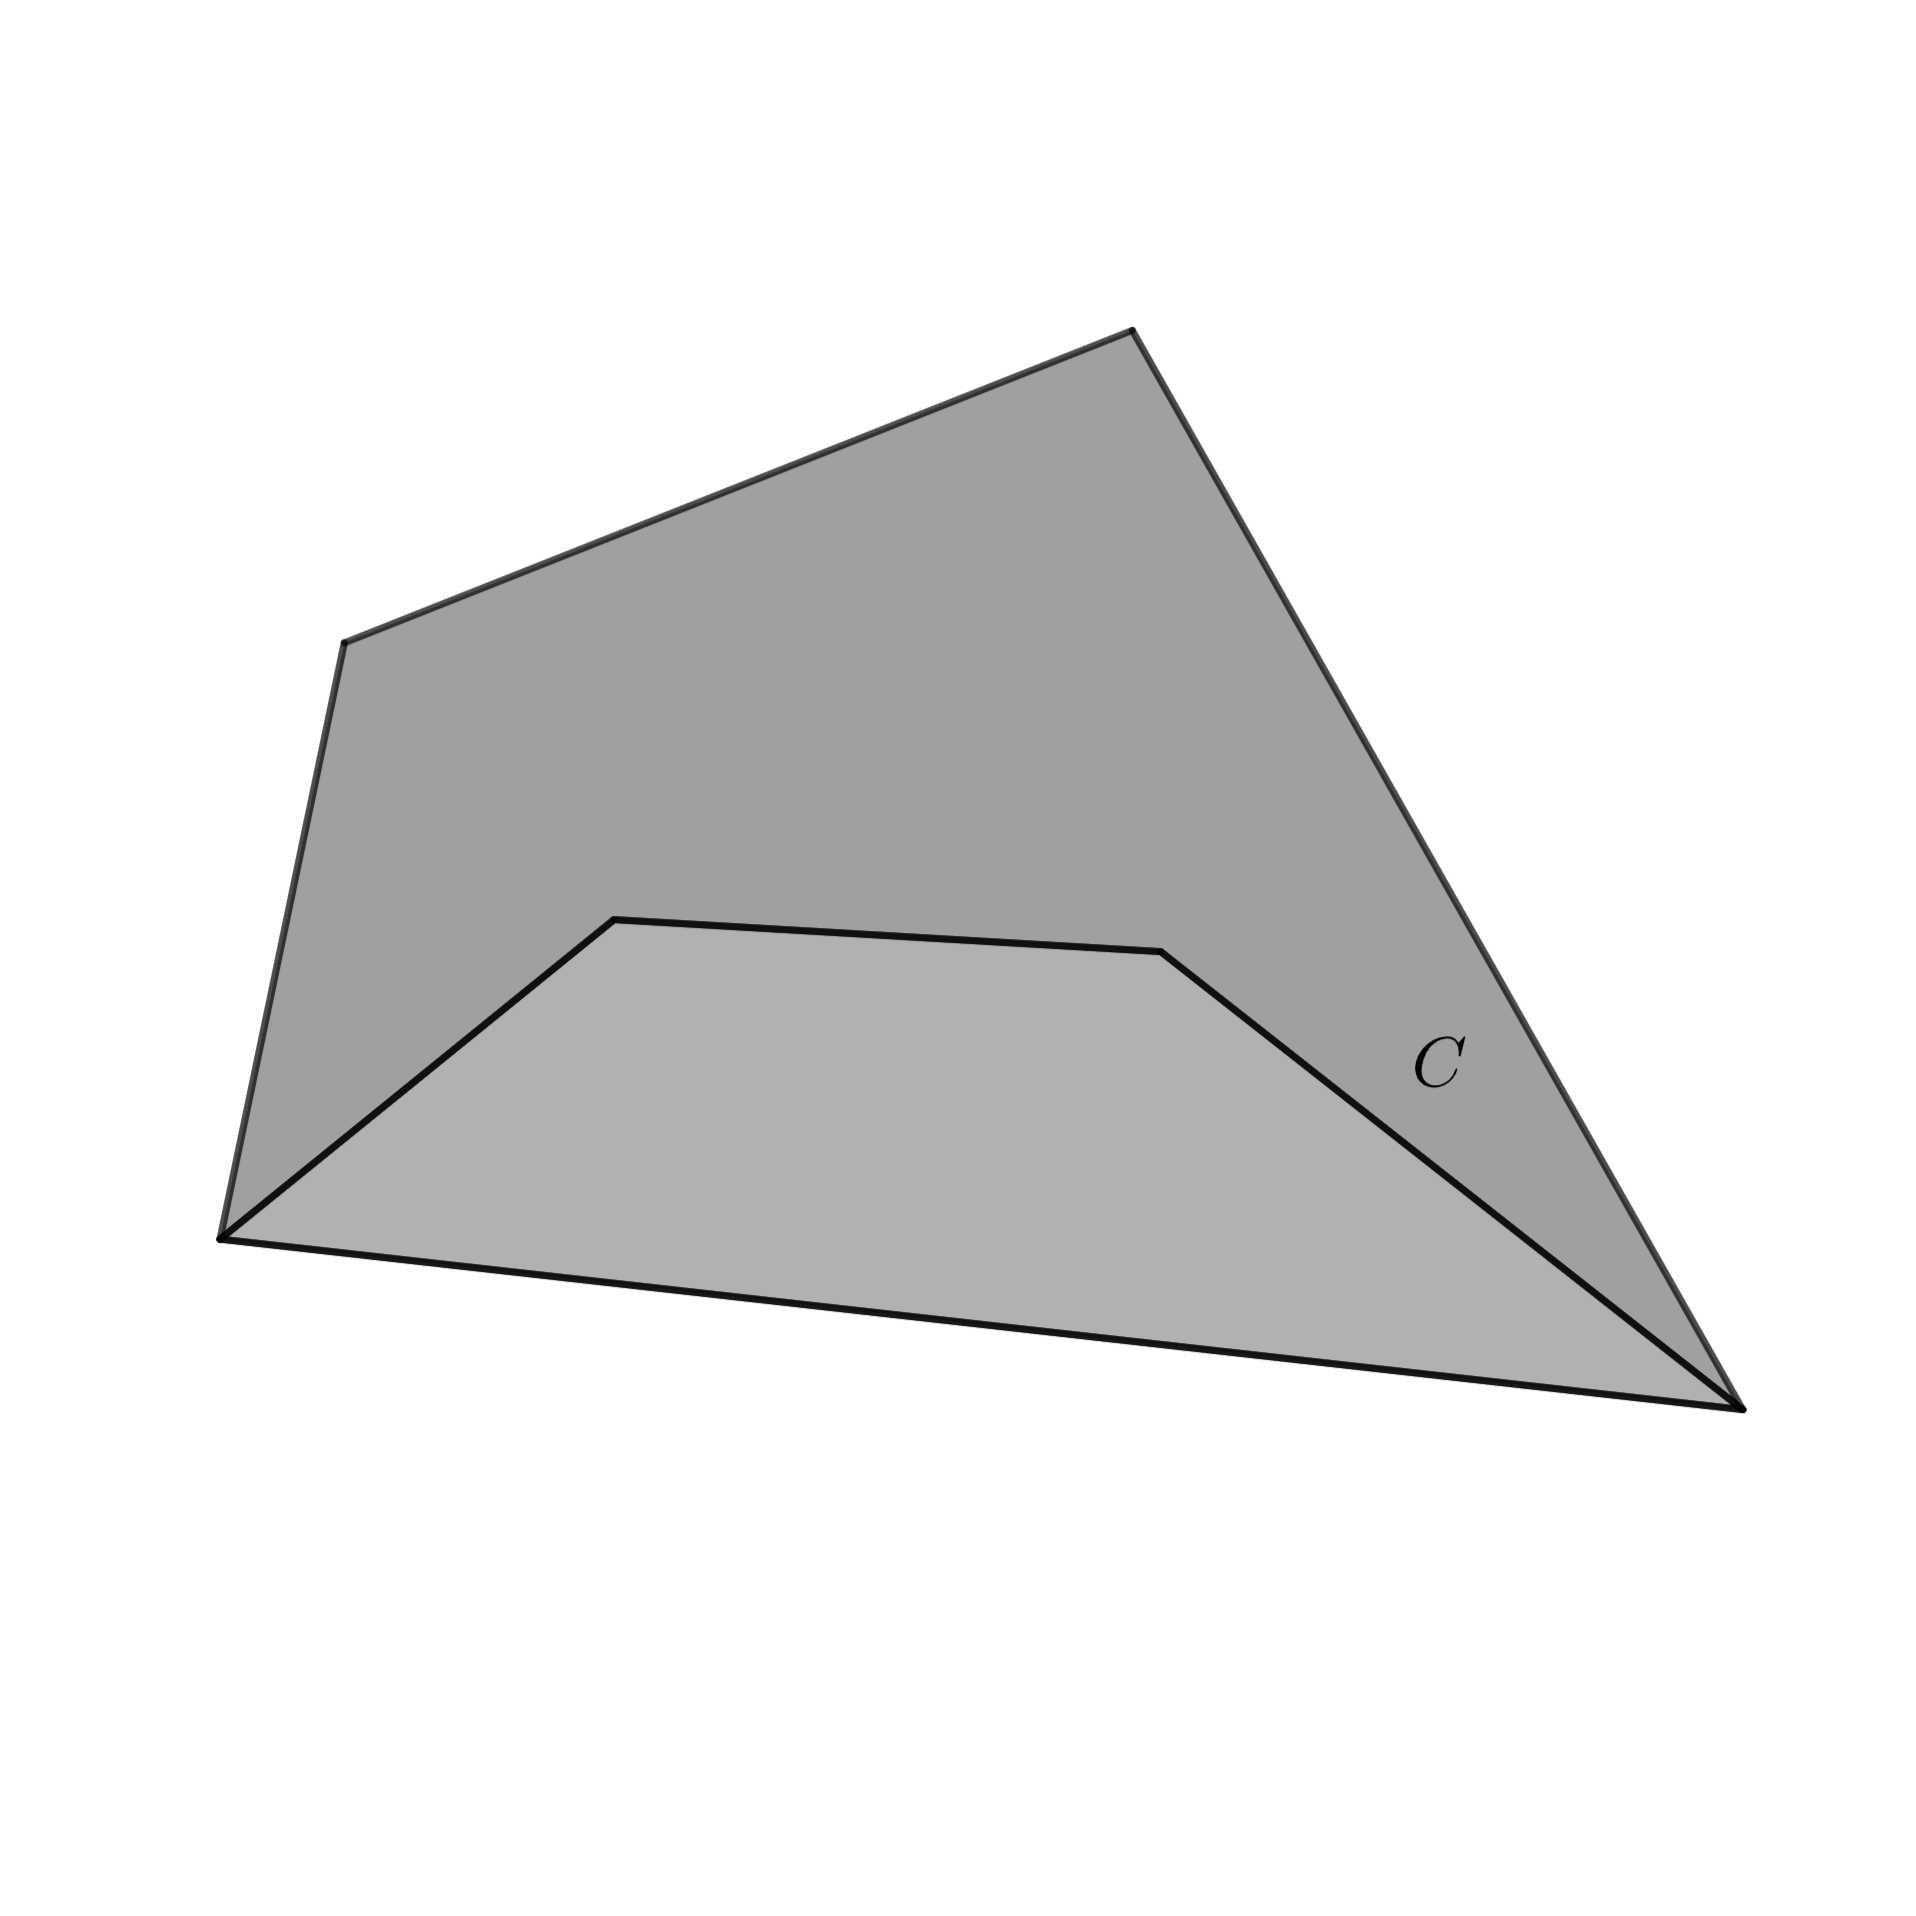
\includegraphics[height = 1.7 in]{ConvexHull.png}
      \captionof{figure}{$\conv C\subseteq\R^2$}
      \label{fig:test2}
    \end{minipage}
    \end{figure}
\end{example}
\smallskip
\begin{definition}[{Relative Interior, \cite[2.1.3]{boyd_vandenberghe_2004}}]
    Let $C\subseteq\R^n$ be a set. The \emph{relative interior} of C can be defined using the affine hull of C as
    \begin{align*}
        \relint C = \{x\in C\ |\ B(x, r) \cap \aff C \subseteq C \text{ for some } r > 0\}
    \end{align*}
    where $B(x, r) = \{y \ |\ ||y-x|| \leq r\}$ is a ball centered at $x$ with radius $r$. In other words, the \emph{relative interior} of a set, $C$, is the set of all points in $C$ from which a ball of non-zero radius can be created in the affine hull of $C$ that is fully contained within C. The relative interior of a convex set is also convex \cite[1.1.1(d)]{bertsekas2009convex}.
\end{definition}
\smallskip
\begin{definition}[{Closure, \cite[2.1.3]{boyd_vandenberghe_2004}}]
    Let $C\subseteq\R^n$ be a set. The \emph{closure} of $C$, denoted $\cl C$, is defined as the set of all points in $C$ and its limit points. The closure of a convex set is also convex \cite[1.1.1(d)]{bertsekas2009convex}.
\end{definition}
\smallskip
\begin{definition}[{Relative Boundary, \cite[2.1.3]{boyd_vandenberghe_2004}}]
    Let $C\subseteq\R^n$ be a set. The \emph{relative boundary} of $C$, denoted $\bd C$, can be expressed as
    \begin{align*}
        \bd C = \cl C \setminus \relint C
    \end{align*}
\end{definition}
\smallskip
\begin{example}
Consider the following set $C$ in $\R^2$ and two points $x_1,x_2\in C$. If it is possible to construct a Euclidean ball of nonzero radius around a point whose intersection with the affine hull of $C$ is fully enclosed within $C$, then the point is part of $C$'s relative interior. In the following figure, $x_2$ is an interior point, while $x_1$ is part of $C$'s relative boundary.
    \begin{figure}[h]
    \centering
    \begin{minipage}{.5\textwidth}
      \centering
      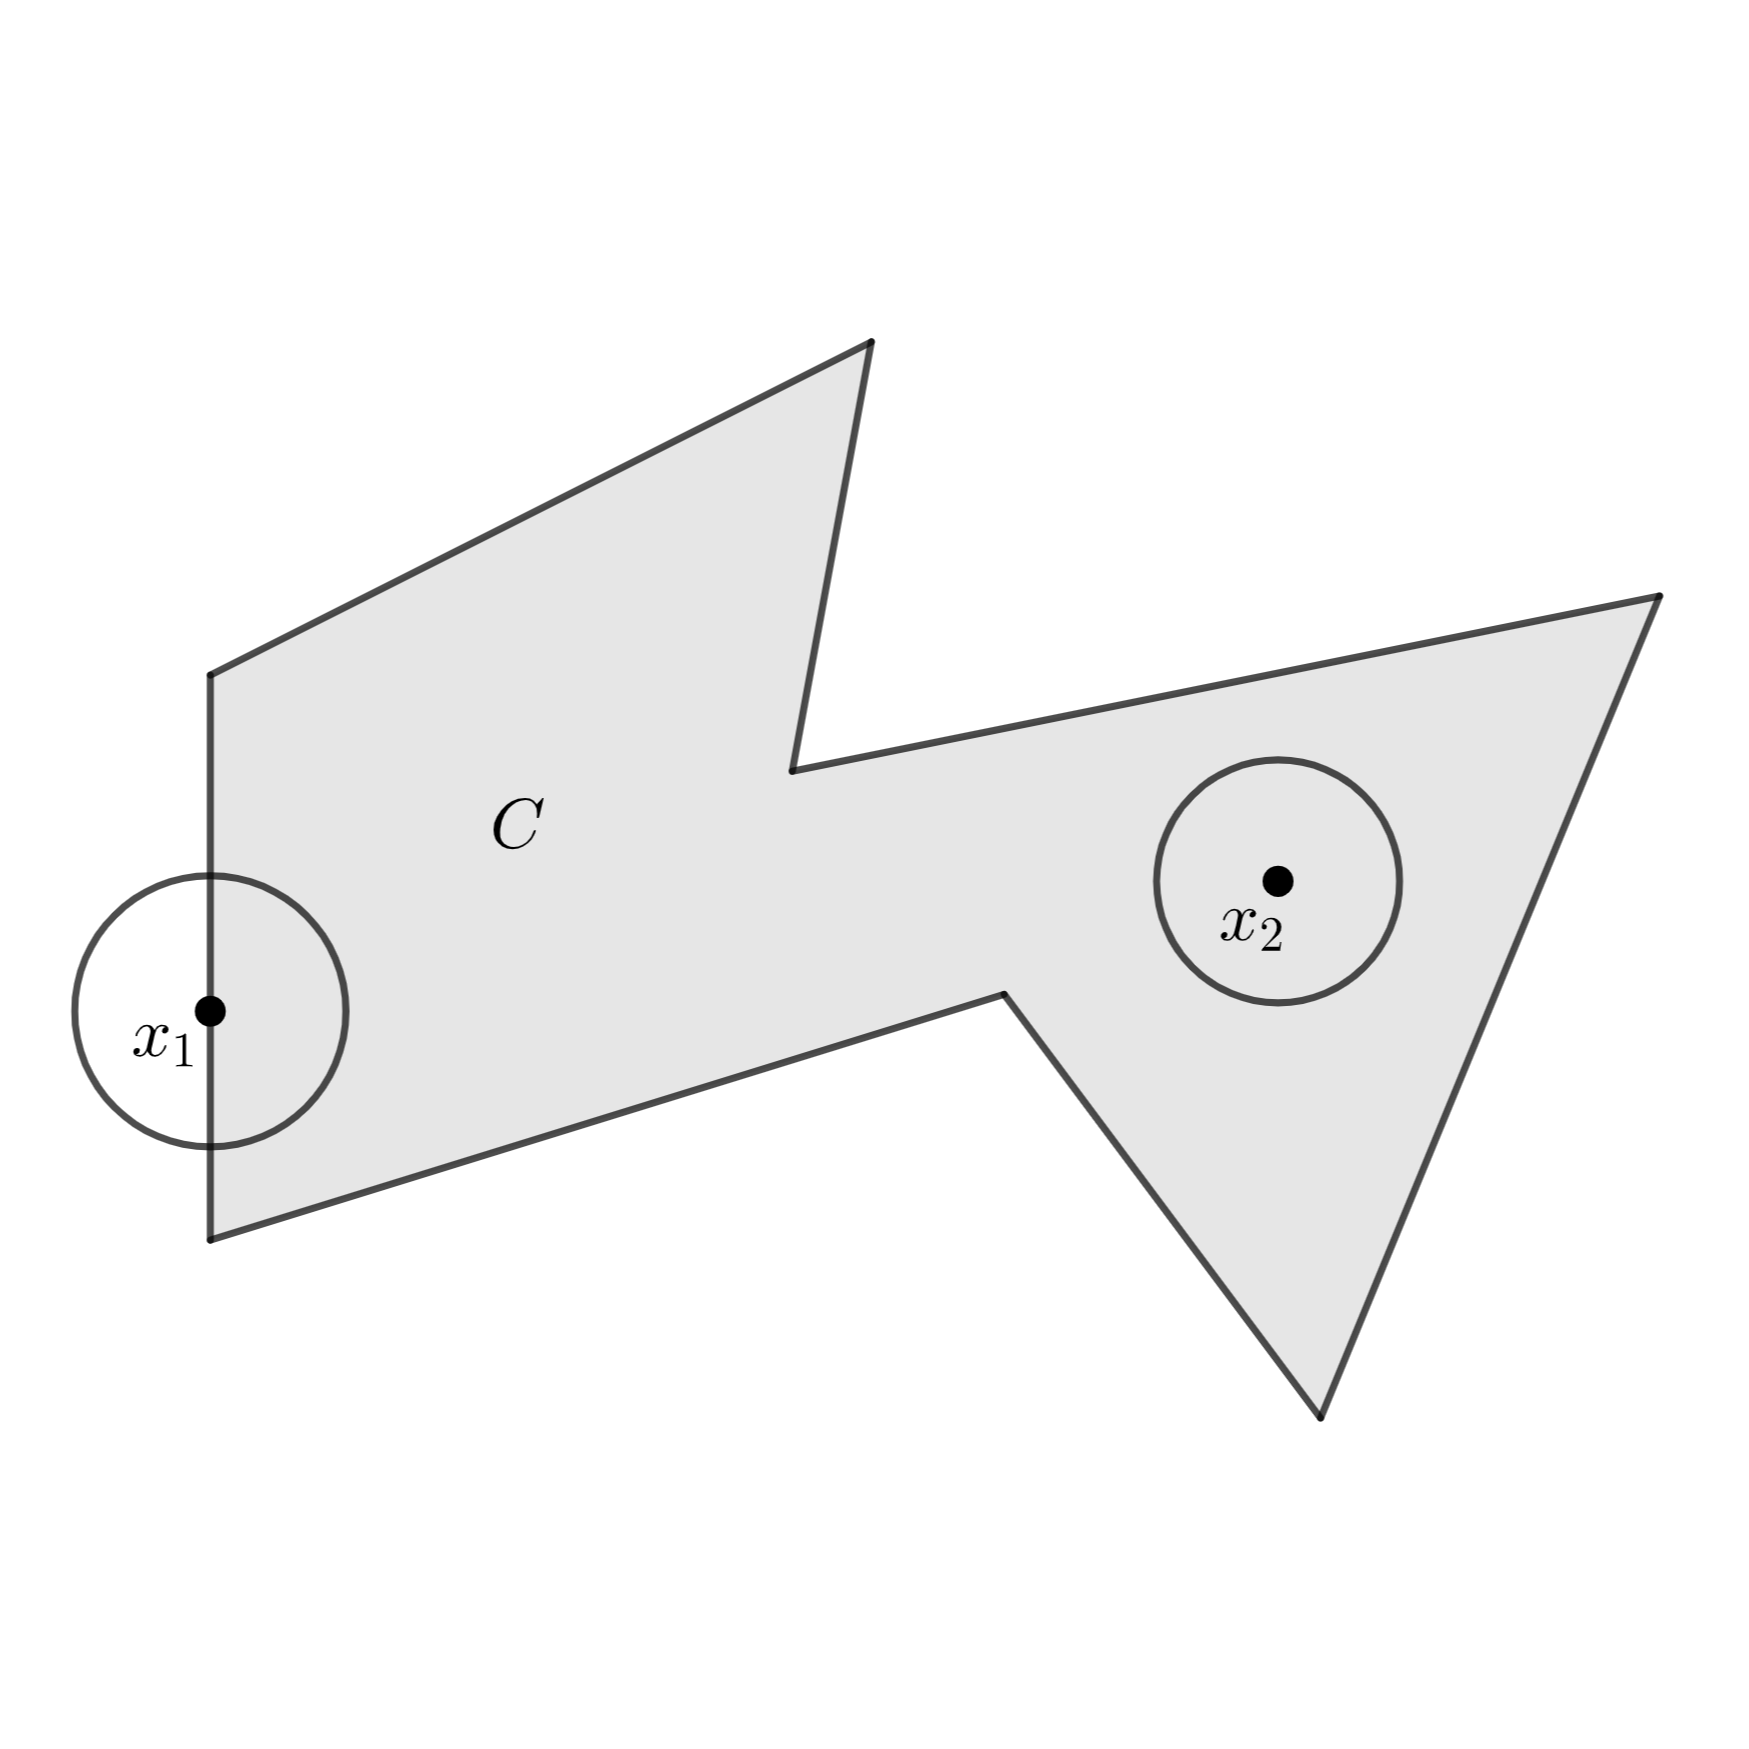
\includegraphics[height = 1.7 in]{relint.png}
      \captionof{figure}{$\relint C$ and $bd C$}
      \label{fig:test1}
    \end{minipage}%
    \end{figure}
\end{example}
\smallskip
\begin{definition}[{Hyperplanes and Halfspaces, \cite[2.2.1]{boyd_vandenberghe_2004}}]
    A \emph{hyperplane} in $\R^n$ is an affine set
    \begin{align*}
        \{x\ |\ \langle a,x\rangle=b\}
    \end{align*}
    where $a\in\R^n$ and $b\in\R$. This relation can be thought of as a set of points with a constant inner product to a vector $a\in\R^n$, \emph{i.e.} a hyperplane that is normal to a vector $a$ with an offset proportional to a scalar $b$ from the origin.

    Thus, hyperplanes are $n-1$ dimensional affine subsets of $\R^n$, which divide the space into two halfspaces
    \begin{align*}
        &\{x\ |\ \langle a,x\rangle \leq b\} &\text{and}& &\{x\ |\ \langle a,x\rangle\geq b\}
    \end{align*}
\end{definition}
\smallskip
\begin{example}
    Consider the inner product space $\R^2$. Hyperplanes in $\R^2$ are one dimensional lines which divide the space into two closed halfspaces as shown in the following figure.
    \begin{figure}[h]
    \centering
    \begin{minipage}{.5\textwidth}
      \centering
      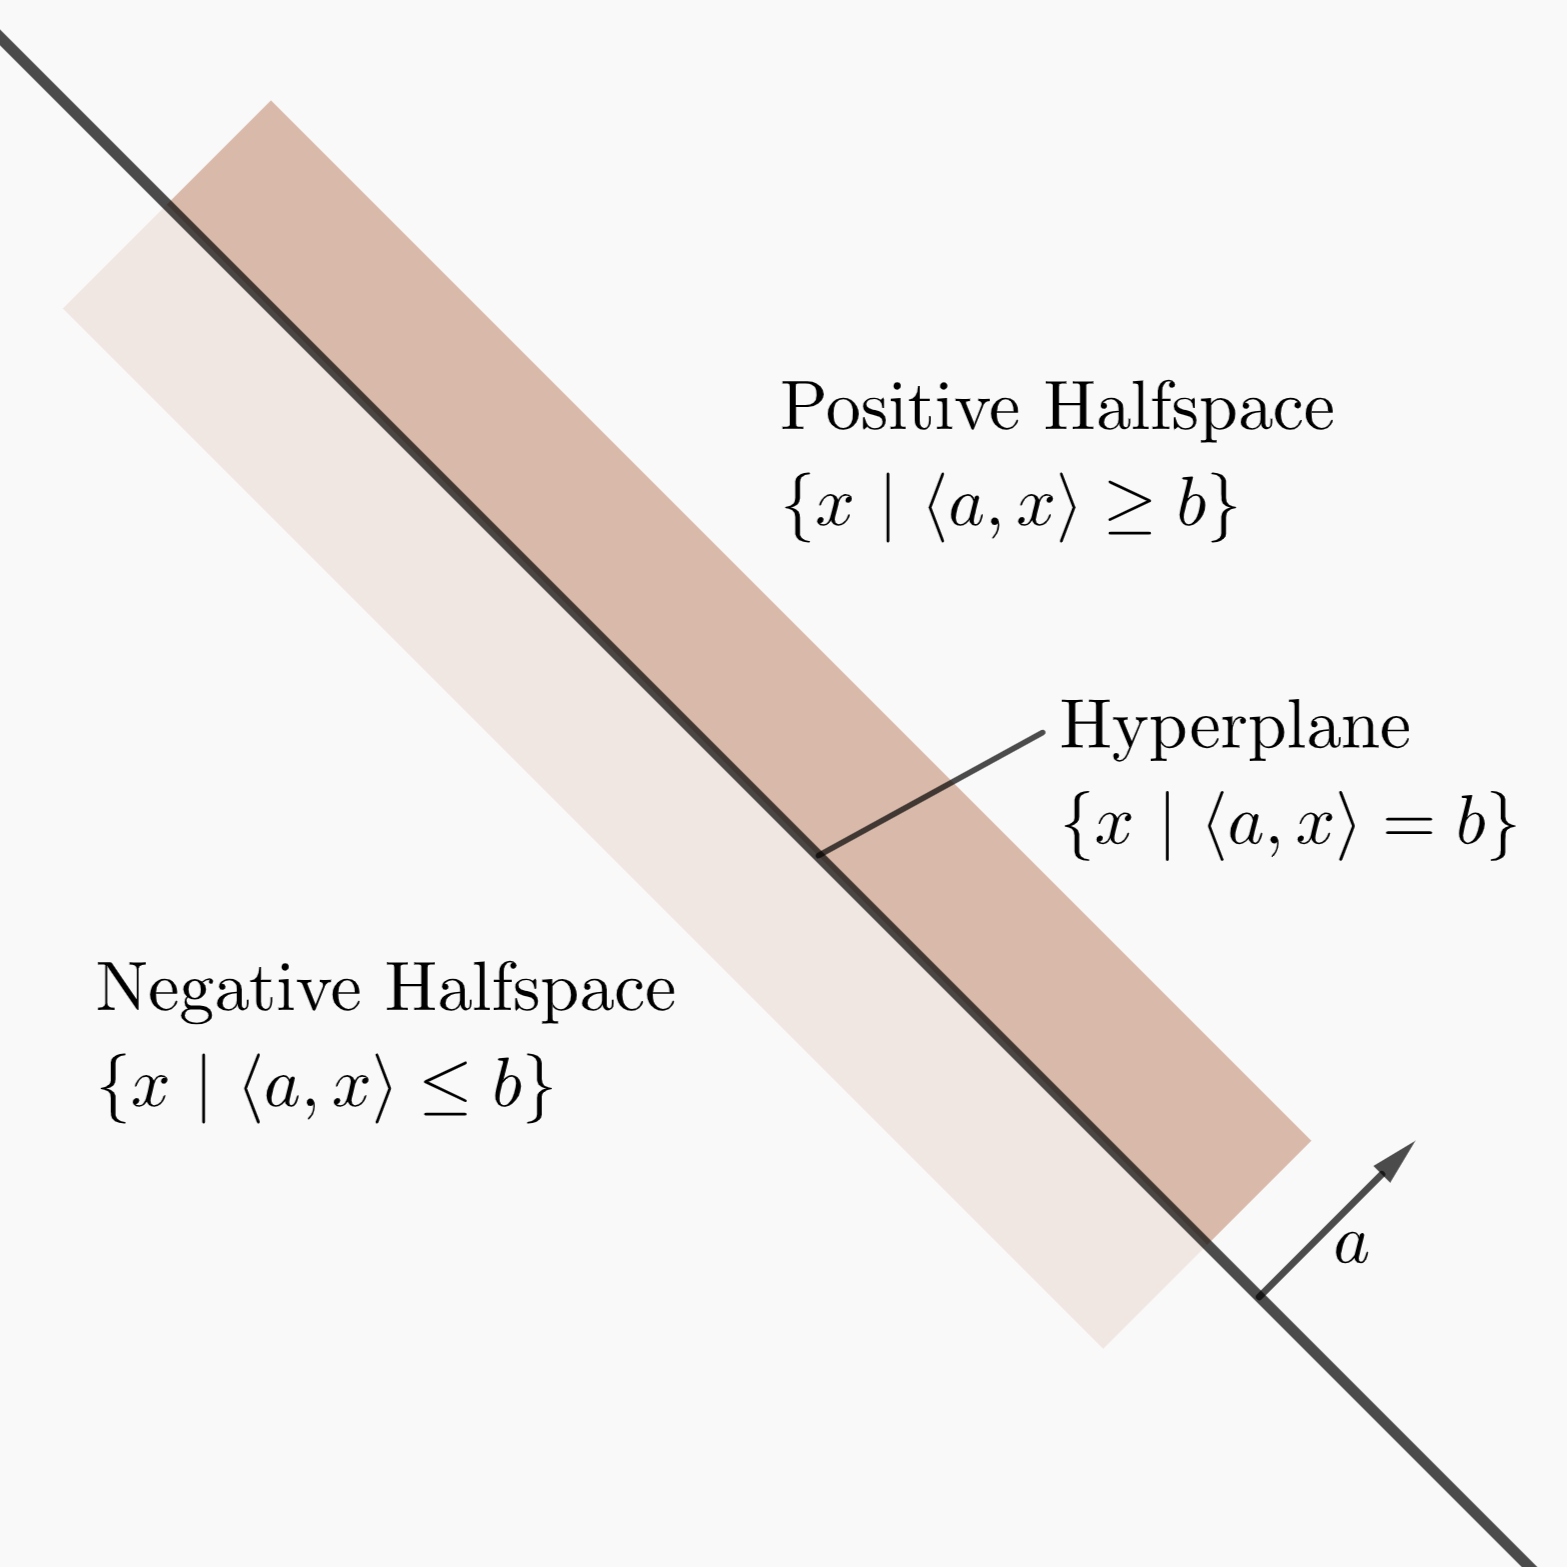
\includegraphics[height = 1.7 in]{halfspaces.png}
      \captionof{figure}{Closed Halfspaces}
      \label{fig:test1}
    \end{minipage}%
    \end{figure}
\end{example}
\smallskip
\begin{definition}[{Separation, \cite[1.5.1]{bertsekas2009convex}}]
    Two sets, $C_1,C_2$ are \emph{separated} by a hyperplane if there exists $a\in\R^n\neq 0$ such that 
    \begin{align*}
        &\langle a,x_1\rangle \leq \langle a,x_2\rangle & \text{for all $x_1\in C_1$, $x_2\in C_2$}
    \end{align*}
\end{definition}
\smallskip
\begin{definition}[{Strict Separation, \cite[1.5.3]{bertsekas2009convex}}]
    Two sets, $C_1,C_2$ are \emph{strictly separated} by a hyperplane if there exists $a\in\R^n\neq 0$ such that
    \begin{align*}
        &\langle a,x_1\rangle < \langle a,x_2\rangle & \text{for all $x_1\in C_1$, $x_2\in C_2$}
    \end{align*}
\end{definition}
\smallskip
\begin{definition}[Supporting Hyperplanes]
    If $x\in\bd C$, the hyperplane separating $C$ and $\{x\}$ is defined as a \emph{supporting hyperplane} at $x$. It is a hyperplane which passes through $x$ and contains $C$ in one of its closed halfspaces.
\end{definition}
\smallskip
\begin{example}
    Consider the closed convex set $C$ in $\R^2$ and $\overline{x}\in\bd C$. A hyperplane can be constructed such that it intersects $\overline{x}$ and fully enclosed the rest of $C$ in one of its halfspaces.
    \begin{figure}[h]
    \centering
    \begin{minipage}{.5\textwidth}
      \centering
      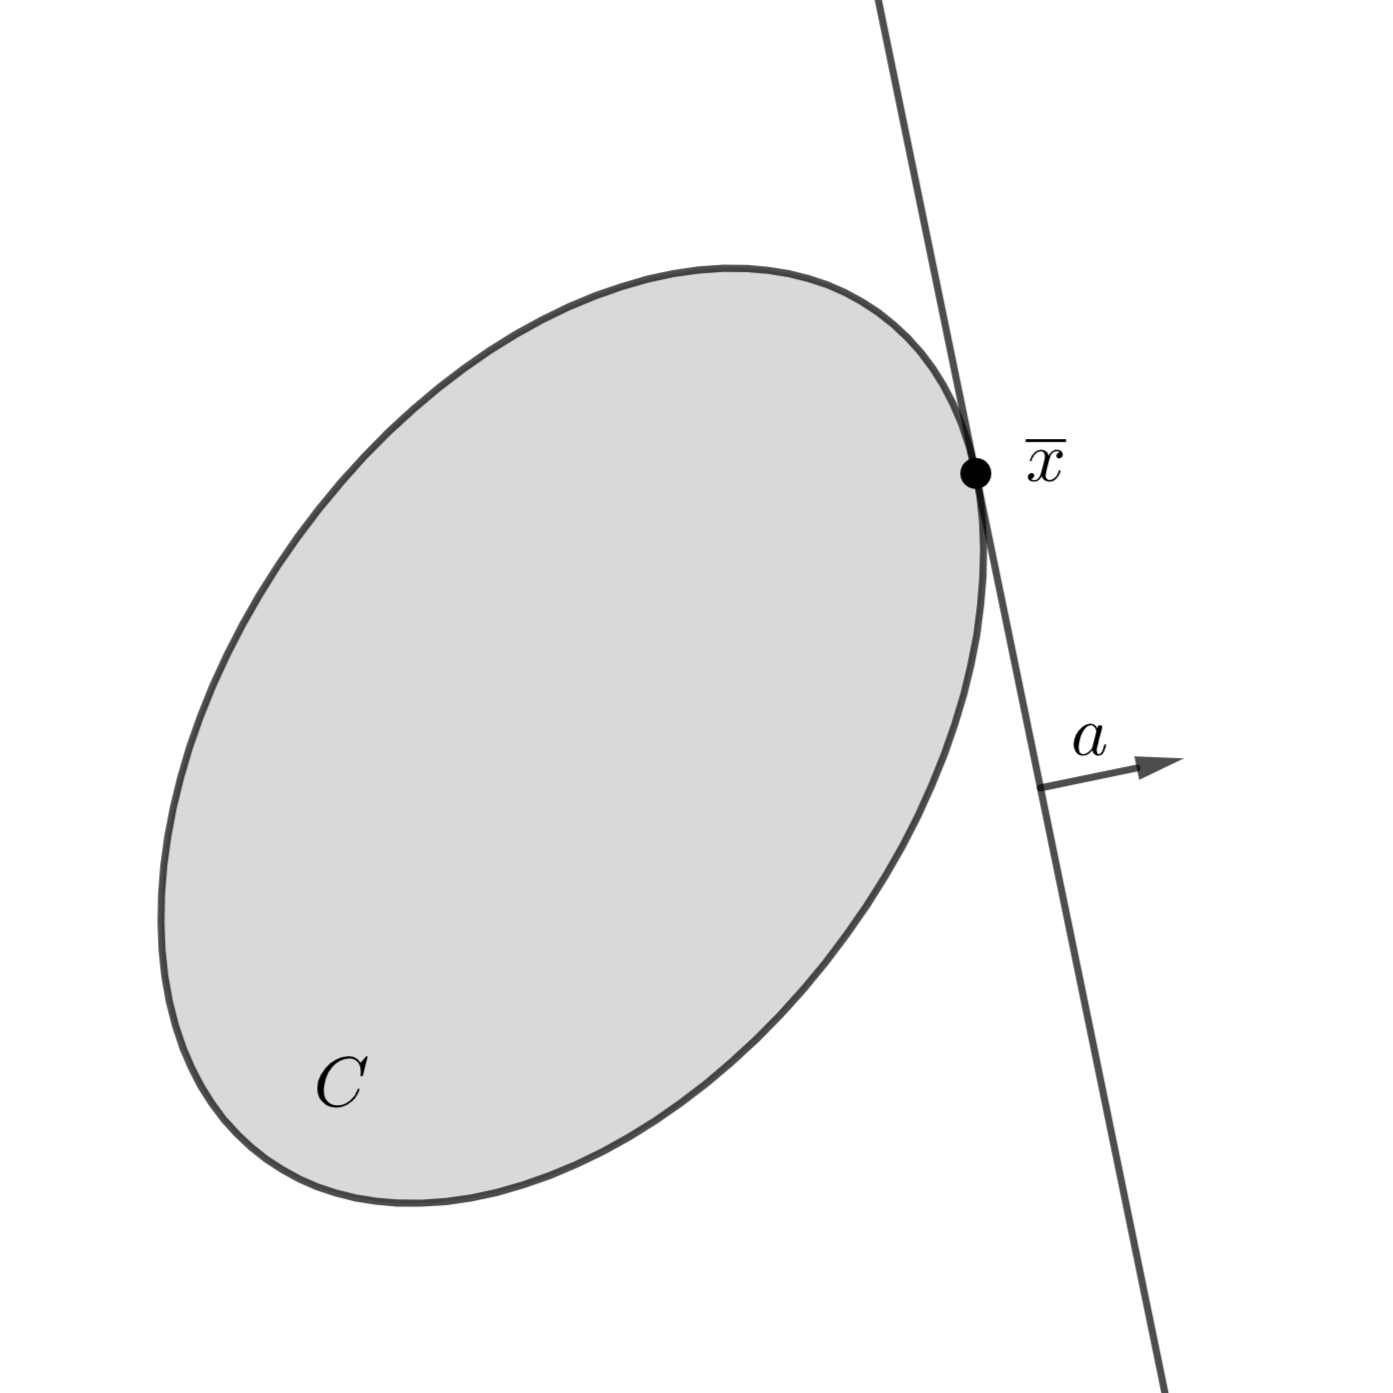
\includegraphics[height = 1.7 in]{supp.png}
      \captionof{figure}{Supp. Hyperplane}
      \label{fig:test1}
    \end{minipage}%
    \end{figure}
\end{example}
\smallskip
\begin{theorem}[{Projection Theorem, \cite[1.1.9]{bertsekas2009convex}}]
    \label{thm:projection}
    Let $C\subseteq\R^n$ be a nonempty, closed convex set, and let $\hat{x}\in\R^n$ be an arbitrary vector. There exists a unique vector $x^*\in C$ such that
    \begin{align*}
        \langle x^* - \hat{x},x-x^*\rangle &\geq 0 & \text{for all $x\in C$}
    \end{align*}
    In other words, the projection of a vector $\hat{x}$ onto a nonempty, closed convex set $C$, denoted $P_C(\hat{x})$, is the unique vector $x^*\in C$ that is closest to $\hat{x}$ for all $x\in C$. A complete proof of the Projection Theorem can be found at \cite[1.1.9]{bertsekas2009convex}.
\end{theorem}
\smallskip
\begin{example}
    Consider the closed convex set $C$ in $\R^2$ and some vector $\hat{x}$ such that $\hat{x}\notin\cl C$. By Theorem \ref{thm:projection}, $P_C(\hat{x})$, the projection of $\hat{x}$ onto $C$, is the unique vector $x^*$ which is closest to $\hat{x}$.
    \begin{figure}[h]
    \centering
    \begin{minipage}{.5\textwidth}
      \centering
      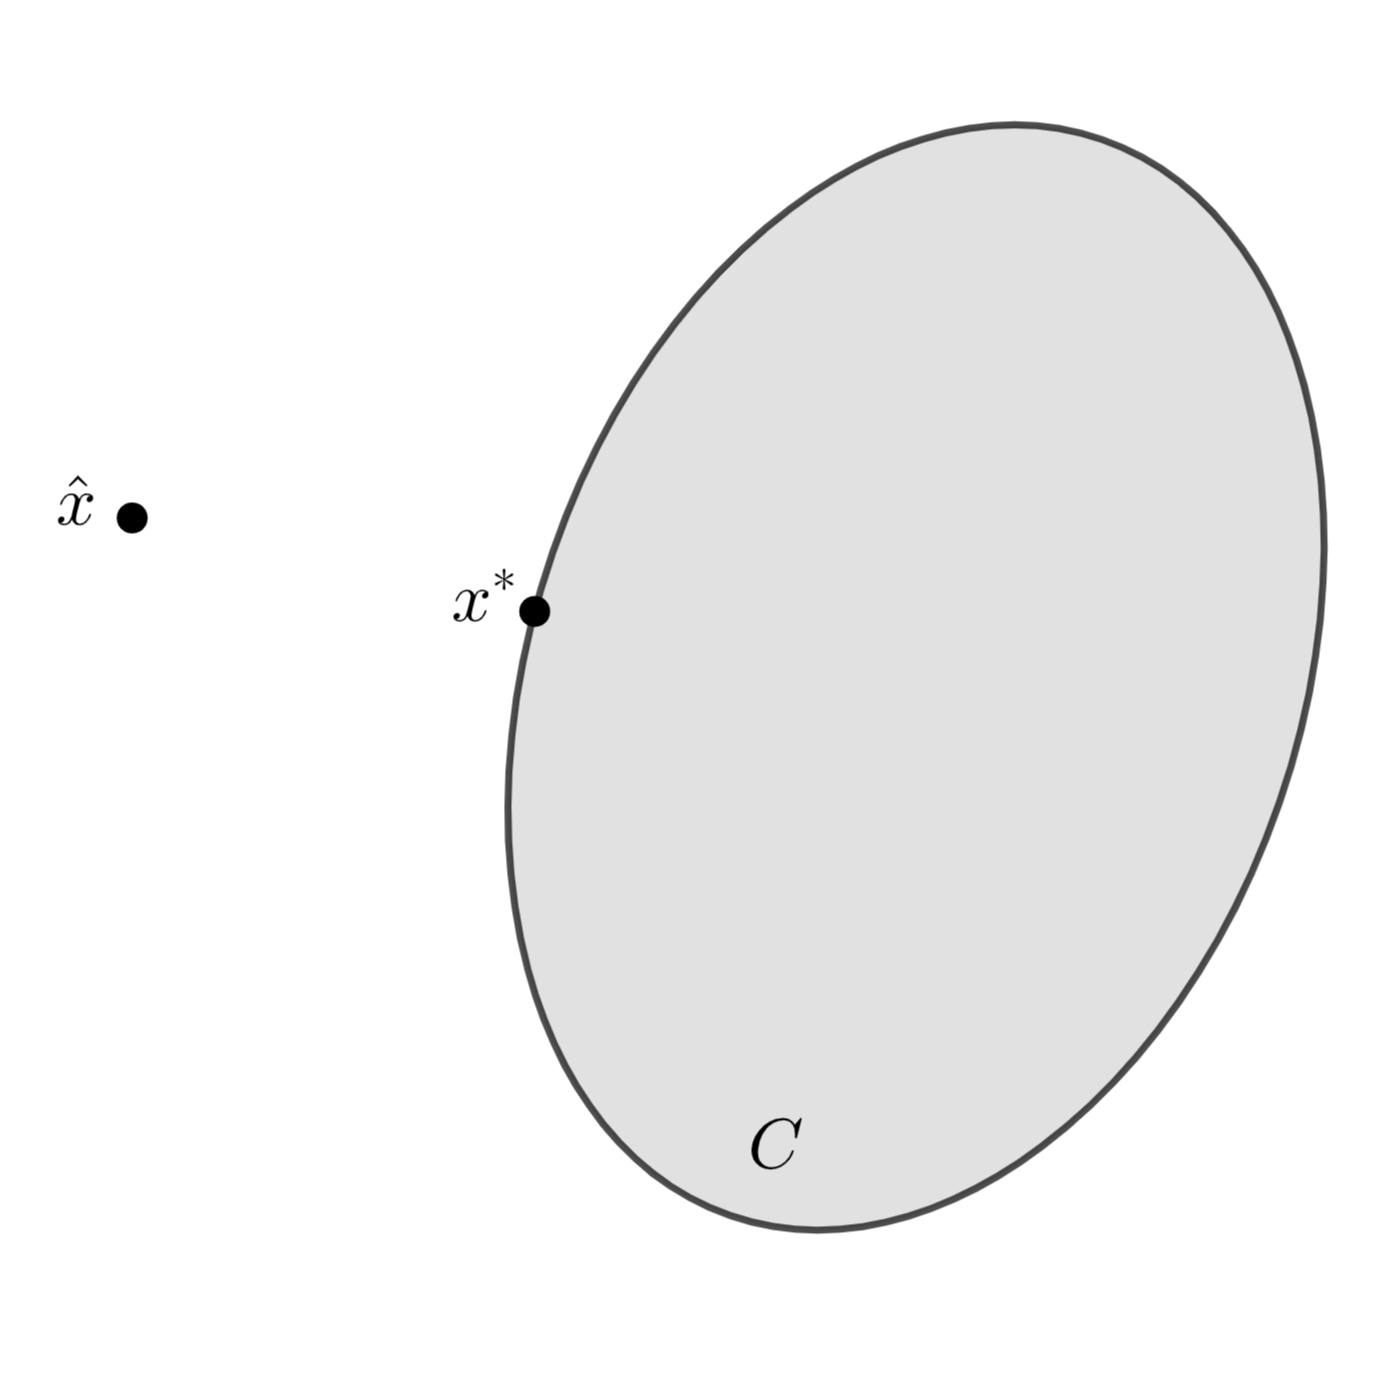
\includegraphics[height = 1.7 in]{proj.png}
      \captionof{figure}{Theorem \ref{thm:projection}}
      \label{fig:test1}
    \end{minipage}%
    \end{figure}
\end{example}
}
%%%%%%%%%%%%%%%%%%%% MAIN THEOREM %%%%%%%%%%%%%%%%%%%%

\section{Main Theorem}
\label{sec:maintheorem}
{
\setlength{\parskip}{8pt}
In order to prove Theorem \ref{thm:main}, we will first prove Theorem \ref{thm:support}, the $\emph{Supporting}$ $\emph{Hyperplane}$ $\emph{Theorem}$.

\begin{maintheorem}[{Supporting Hyperplane Theorem, \cite[1.5.1]{bertsekas2009convex}}]
    \label{thm:support}
     Let $C\subseteq\R^n$ be a nonempty, closed convex set, and let $\overline{x}\in\R^n$ such that $\overline{x}\notin\relint C$. Then there exists $a\in\R^n\neq 0$ such that
    \begin{align*}
        &\langle a,\overline{x}\rangle \leq\langle a,x\rangle & \text{for all $x\in C$}
    \end{align*}
    \emph{i.e.} if $\overline{x}$ is not in the interior of $C$, there exists a hyperplane which passes through $\overline{x}$ and contains $C$ in one of its closed halfspaces.
    \begin{proof}
        We have that $\cl C$, the closure of $C$, is also convex since $C$ is convex. Let $\{x_k\}$ be a sequence of vectors such that $x_k\rightarrow\overline{x}$ while $x_k\notin\cl C$ for all $k$. We have the existence of such a sequence because $\overline{x}$ is not in the interior of $C$, which implies that it is also not in the interior of $\cl C$.

        Let $\hat{x}_k = P_C(x_k)$, \emph{i.e.} the projection of $x_k$ onto $C$. By the Projection Theorem \ref{thm:projection}, we have that
        \begin{align*}
            &\langle \hat{x}_k - x_k, x - \hat{x}_k\rangle \geq 0 & \text{for all $x\in\cl C$}
        \end{align*}
        Thus, for all $x\in\cl C$ and $k\in\N$, we have
        \begin{align*}
            \langle \hat{x}_k - x_k, x\rangle -\langle \hat{x}_k - x_k,\hat{x}_k\rangle &\geq 0\\
            \langle \hat{x}_k - x_k, x\rangle &\geq \langle \hat{x}_k - x_k,\hat{x}_k\rangle\\
            \langle \hat{x}_k - x_k, x\rangle &\geq \langle \hat{x}_k - x_k,\hat{x}_k-x_k\rangle + \langle \hat{x}_k - x_k,x_k\rangle\\
            \langle \hat{x}_k - x_k, x\rangle &\geq ||\hat{x}_k - x_k||^2 + \langle \hat{x}_k - x_k,x_k\rangle\\
            \langle \hat{x}_k - x_k, x\rangle &\geq \langle \hat{x}_k - x_k,x_k\rangle
        \end{align*}
        Let $a_k = \frac{\hat{x}_k-x_k}{||\hat{x}_k-x_k||}$, the unit vector from $x_k$ to $\hat{x}_k$. We can now write this relation as
        \begin{align*}
            &\langle a_k,x\rangle \geq \langle a_k,x_k\rangle &\text{for all $x\in\cl C$, $k\in\N$}
        \end{align*}
        We have that $||a_k||=1$ for all $k\in\N$, which implies that $\{a_k\}$ contains a subsequence that converges to some $a\neq 0$. Therefore, by taking the limit of this sequence as $k\rightarrow\infty$, we obtain
        \begin{align*}
            &\langle a,x\rangle \geq \langle a,\overline{x}\rangle &\text{for all $x\in\cl C$}
        \end{align*}
    \end{proof}
\end{maintheorem}
\smallskip
\begin{example}[{\cite[1.5.3]{bertsekas2009convex}}]
    The following figure depicts the proof of Theorem \ref{thm:support} for the specific case in which $\overline{x}\in\cl C$. We can create a sequence of vectors $\{x_k\}$ such that each $x_k\notin\cl C$ and $x_k\rightarrow \overline{x}$. Each $x_k$ is projected onto $C$ to corresponding points $\hat{x}_k$. For each $k\in\N$, we can construct a hyperplane that is orthogonal to the line segment connecting each $x_k$ to its projection $\hat{x}_k$. In this case, these hyperplanes will converge to a supporting hyperplane through $\overline{x}$ on $C$.
    \begin{figure}[h]
    \centering
    \begin{minipage}{.5\textwidth}
      \centering
      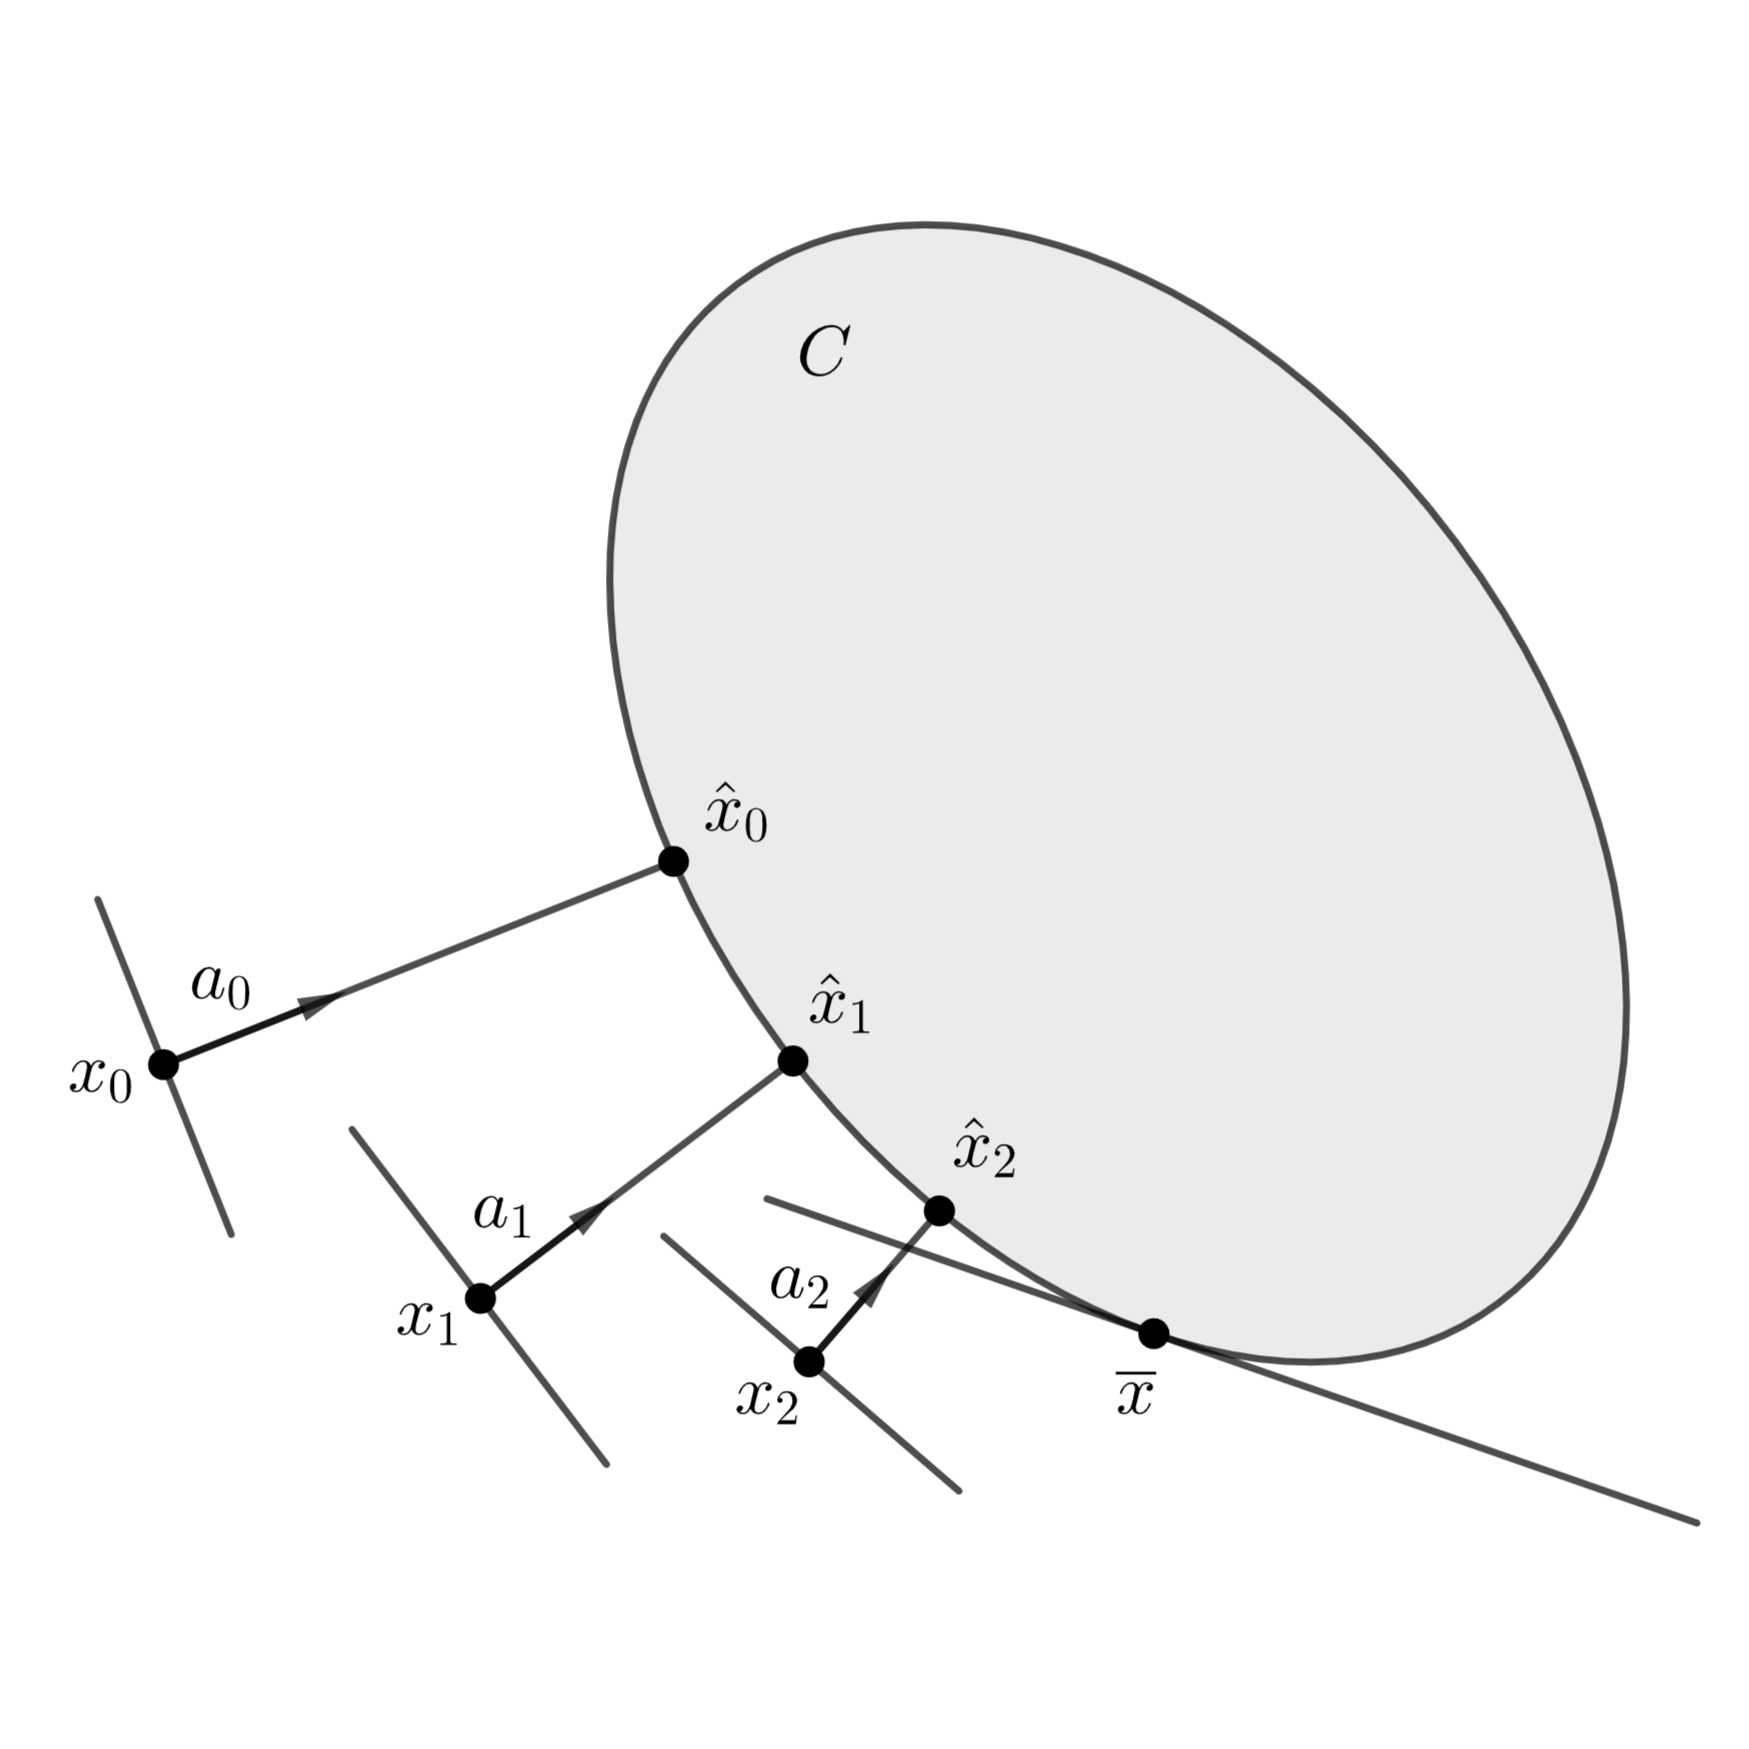
\includegraphics[height = 1.7 in]{thoeremB.png}
      \captionof{figure}{Theorem \ref{thm:support}}
      \label{fig:test1}
    \end{minipage}%
    \end{figure}
\end{example}
\smallskip
\begin{maintheorema}[{Separating Hyperplane Theorem, \cite[1.5.2]{bertsekas2009convex}}]
   Let $C_1, C_2 \subseteq\R^n$ be two nonempty disjoint convex sets. Then there exists $a\in\R^n\neq 0$ such that 
   \begin{align*}
    &\langle a,x_1\rangle \leq \langle a,x_2\rangle &\text{for all $x_1 \in C_1$ and $x_2 \in C_2$}
   \end{align*}
   In other words, there exists a hyperplane separating $C_1$ and $C_2$.
   \begin{proof}
       Let $C$ be the convex set defined by
       \begin{align*}
           C = C_2 - C_1 = \{x\ |\ x= x_2 - x_1,\ x_1\in C_1,\ x_2\in C_2\}
       \end{align*}
       Since $C_1$ and $C_2$ are disjoint, for all $x_1\in C_1$ and $x_2\in C_2$, $x_1\neq x_2$. Thus, we have that $0\notin C$. By Theorem \ref{thm:support}, there exists $a\in\R^n\neq 0$ such that
       \begin{align*}
           &\langle a,0\rangle \leq \langle a,x\rangle &\text{for all $x\in C$}
       \end{align*}
       Hence, for all $x\in C$, $x_1\in C_1$, and $x_2\in C_2$, we have that
       \begin{align*}
           0 &\leq \langle a,x\rangle\\
           0 &\leq \langle a,x_2-x_1\rangle\\
           0 &\leq \langle a,x_2\rangle - \langle a,x_1\rangle\\
           \langle a,x_1\rangle &\leq \langle a,x_2\rangle
       \end{align*}
   \end{proof}
\end{maintheorema}
\smallskip
\begin{example}[{\cite[1.5.1]{bertsekas2009convex}}]
    Consider the following two nonempty disjoint convex sets $C_1,C_2\subseteq\R^2$. As proven in Theorem \ref{thm:main}, it is possible to separate both sets with a hyperplane normal to some $a\in\R^2\neq 0$.
    \begin{figure}[h]
    \centering
    \begin{minipage}{.5\textwidth}
      \centering
      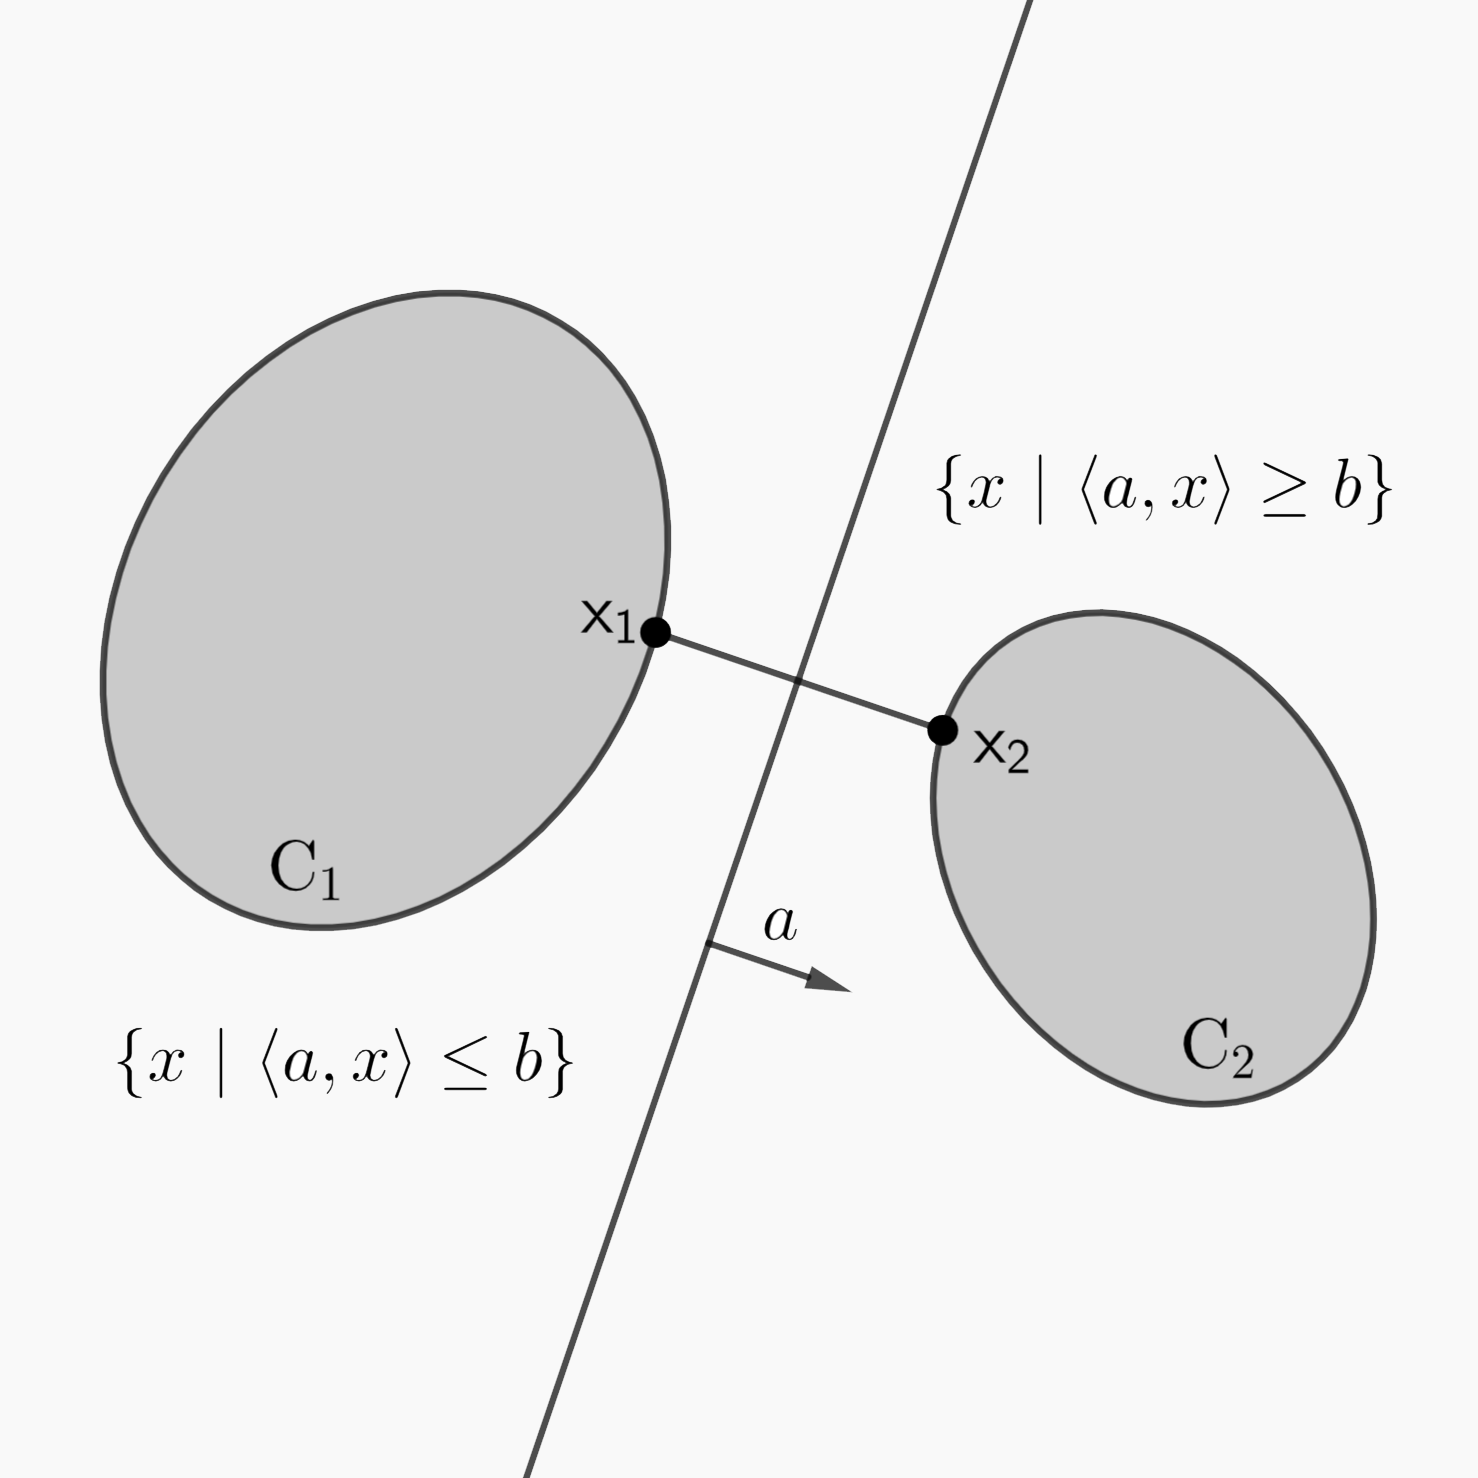
\includegraphics[height = 1.7 in]{separating hyperplane.png}
      \captionof{figure}{Theorem \ref{thm:main}}
      \label{fig:test1}
    \end{minipage}%
    \end{figure}
\end{example}
}
%%%%%%%%%%%%%%%%%%%% APPLICATIONS %%%%%%%%%%%%%%%%%%%%

\section{Applications}
\label{sec:applications}
{
\setlength{\parskip}{8pt}
We now give an example of an application of Theorem \ref{thm:main}  in proving the \emph{strict separation} of two sets:
\begin{corollary}[{Strict Hyperplane Separation, \cite[1.5.3]{bertsekas2009convex}}]
    Let $C_1,C_2\subseteq\R^n$ be two disjoint, nonempty, closed convex sets. There exists a hyperplane which strictly separates $C_1$ and $C_2$ under any one of the following three conditions:
    
    \onehalfspacing
    (1) $C_2 - C_1$ is closed.\\
    (2) $C_1$ is closed, and $C_2$ is compact.\\
    (3) $C_1$ and $C_2$ are polyhedral.
    \singlespacing
    \begin{proof}
        We will prove the result under condition (1). The result will then follow under conditions (2) and (3) because these conditions imply condition (1) \cite[1.4.14]{bertsekas2009convex}.

        Assume that $C_2-C_1$ is closed. Consider the vector of minimum norm in $C_2-C_1$, which is the projection of the origin \cite[1.1.9]{bertsekas2009convex}. This vector will be of the form $\overline{x}_2 - \overline{x}_1$, where $\overline{x}_1\in C_1$ and $\overline{x}_2\in C_2$. Let
        \begin{align*}
            &a = \frac{\overline{x}_2 - \overline{x}_1}{2},& &\overline{x} =  \frac{\overline{x}_1 + \overline{x}_2}{2}, &b=\langle a,\overline{x}\rangle
        \end{align*}
        Since $C_1$ and $C_2$ are disjoint, we have that $x_1\neq x_2$ for all $x_1\in C_1$ and $x_2\in C_2$. Hence, we have that $a\neq 0$. We will now show that the hyperplane
        \begin{align*}
            \{x\ |\ \langle a,x\rangle = b\}
        \end{align*}
        strictly separates $C_1$ and $C_2$. By the definition of strict separation, this means
        \begin{align*}
            &\langle a,x_1\rangle < b < \langle a,x_2\rangle &\text{for all $x_1\in C_1$, $x_2\in C_2$}
        \end{align*}
        We have that $\overline{x}_1$ is the projection of $\overline{x}_2$ onto $\cl C_1$, the closure of $C_1$. If this was not the case, we would have the existence of another vector $x_1\in C_1$ such that $||\overline{x}_2 - x_1|| < ||\overline{x}_2 - \overline{x}_1||$, but this contradicts the condition that $x_2 - x_1$ is the vector of minimum norm in $C_2 - C_1$.

        Thus, by the Projection Theorem \ref{thm:projection}, we have that
        \begin{align*}
            &\langle \overline{x}_2 - \overline{x}_1, x_1 - \overline{x}_1\rangle \leq 0 &\text{for all $x_1\in C_1$}
        \end{align*}
        Since $a$ can also be expressed as $\overline{x} - \overline{x}_1$, \emph{i.e.} the vector pointing from $\overline{x}_1$ to the average of $\overline{x}_1$ and $\overline{x}_2$,
        \begin{align*}
            \langle a,x_1-\overline{x}_1\rangle &\leq 0\\
            \langle a,x_1\rangle - \langle a,\overline{x}_1\rangle &\leq 0\\
            \langle a,x_1\rangle &\leq \langle a,\overline{x}_1\rangle
        \end{align*}
        At this point, we will show that $\langle a,x_1\rangle < b$, which is half of the desired equation.
        \begin{align*}
            \langle a,x_1\rangle &\leq \langle a,\overline{x}\rangle + \langle a,\overline{x}_1 - \overline{x}\rangle\\
            \langle a,x_1\rangle &\leq \langle a,\overline{x}\rangle + \langle a,-a\rangle\\
            \langle a,x_1\rangle &\leq \langle a,\overline{x}\rangle - ||a||^n\\
            \langle a,x_1\rangle &\leq b - ||a||^n\\
            \langle a,x_1\rangle &< b
        \end{align*}
        The right hand side of the equation, $\langle a,x_2\rangle > b$, can be proven using a similar approach.
    \end{proof}
\end{corollary}
}
%%%%%%%%%%%%%%%%%%%% FUTURE DIRECTIONS %%%%%%%%%%%%%%%%%%%%

\section{Future Directions}
\label{sec:futuredirections}
{
\setlength{\parskip}{8pt}
\begin{question}
    Can Theorem \ref{thm:main} be applied to infinite-dimensional vector spaces?
\end{question}

\begin{question}
    More generally, can hyperplane separation be defined in infinite-dimensional vector spaces?
\end{question}

\begin{question}
    How can Theorem \ref{thm:main} be generalized to the Hahn-Banach Separation Theorem?
\end{question}
}
%%%%%%%%%%%%%%%%%%%% REFERENCES %%%%%%%%%%%%%%%%%%%%

\nocite{*}
\bibliographystyle{abbrv}
\bibliography{citations}

\end{document}